\chapter{Tests}
This chapter includes test descriptions and results to validate the design against the requirements. First, the two directional antennas are tested to find their gain and ensure, that the transmitter and receiver have their maximum gain at the same frequency. Finally, the full test of the beam steering and transmitter locator is tested with the transmitter fixed at a known location in the test area.

\section{Test of Horn Antenna S-Parameters} \label{s:sparam_test}
The aim of this test is to test the reflection coefficient of the receiving antenna. The measurement will be used to choose the resonance frequency for the acceptance test.

\subsubsection{Equipment}
To perform the test the following equipment is needed:
\begin{itemize}
    \item Rohde \& Schwarz ZNA Vector Network Analyzer (\SI{10}{\mega\hertz}-\SI{43.5}{\giga\hertz})
    \item Rohde \& Schwarz ZN-Z54 Calibration Unit (\SI{9}{\kilo\hertz}-\SI{40}{\giga\hertz})
    \item \SI{50}{\ohm} antenna cable
\end{itemize}

\subsubsection{Procedure}
The test is performed once. The following explains the procedure for the test:
\begin{enumerate}
    \item Add power to VNA, connect antenna cable to VNA and Calibration unit.
    \item Make calibration test by choosing \textit{Cal $\rightarrow$ Quick Start Calibration $\rightarrow$ Apply} on the VNA.
    \item Disconnect antenna cable and reconnect to DUT.
    \item Set start and stop frequencies. 
    \item Ensure that VNA measures $S_{11}$-parameter by choosing \textit{Meas $\rightarrow$ $S_{11}$}.
\end{enumerate}
The receiver antenna is a horn antenna which is designed to work in the spectrum from \SI{4}{\giga\hertz} to \SI{7}{\giga\hertz}. The measurement is performed in the spectrum \SI{3}{\giga\hertz} to \SI{8}{\giga\hertz} in order to encaosulate the entire antenna frequency spectrum, with steps of \SI{25}{\mega\hertz}. 

\subsubsection{Result}
The following figure shows $S_{11}$ at the measured frequencies
\begin{figure}[H]
    \centering
    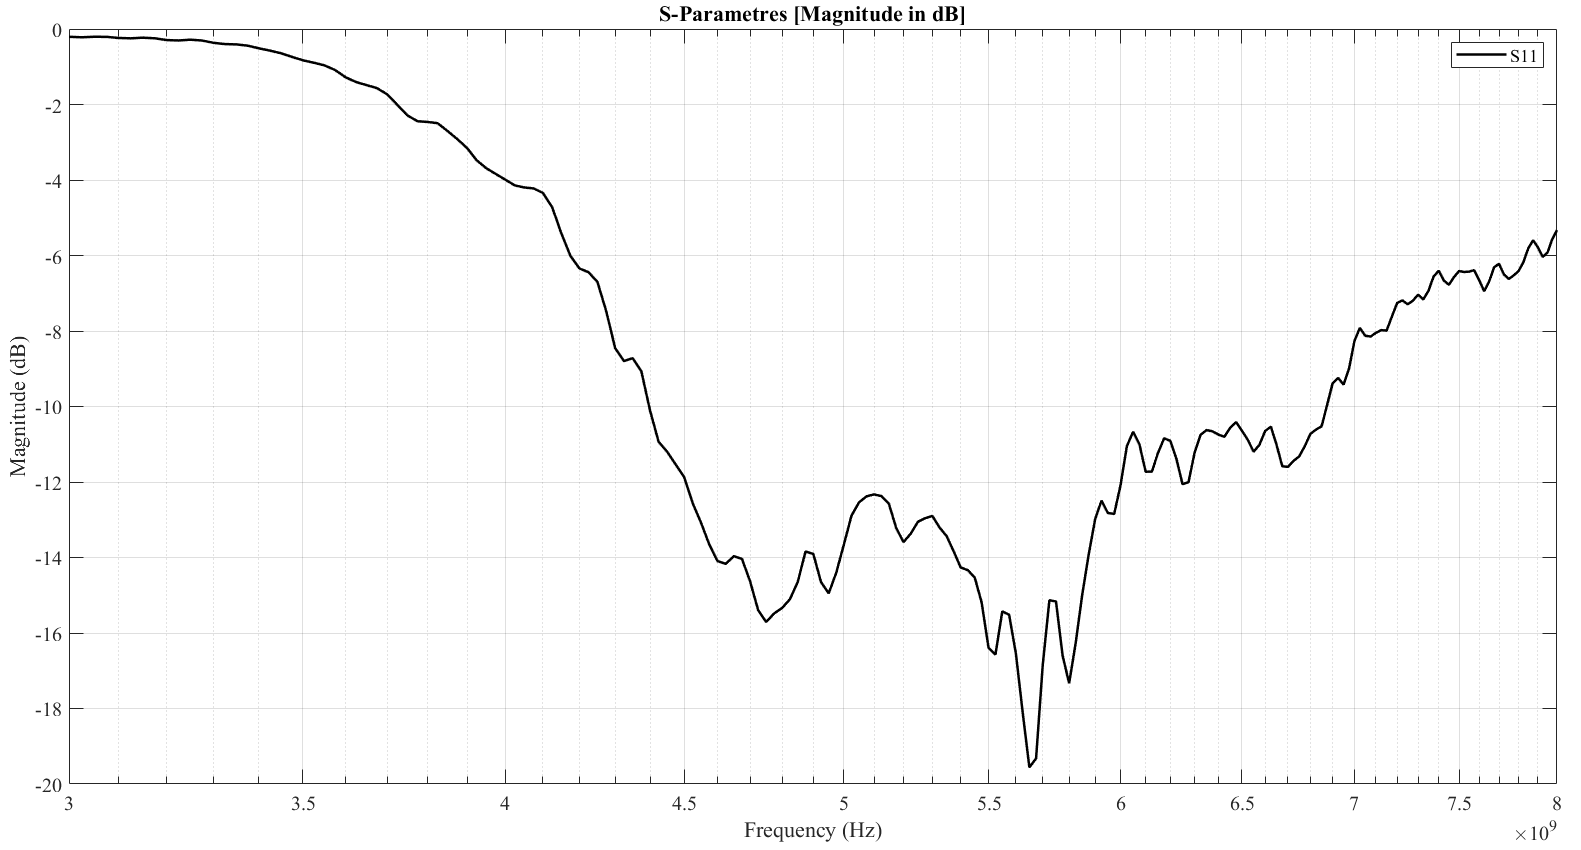
\includegraphics[width=1\textwidth]{figures/s11_meas.png}
    \caption{Measured $S_{11}$-parameter from \SI{3}{\giga\hertz} to \SI{8}{\giga\hertz}.} \label{fig:s11_meas}
\end{figure}
It can be seen that the antenna has a maximum $S_{11}$ magnitude of \SI{-19.56}{\decibel} at \SI{5.65}{\giga\hertz}. This gives a reflection coefficient of $\Gamma = 10^{-19.56/20} = 0.11$. Almost \SI{1}{\giga\hertz} away at \SI{4.75}{\giga\hertz} the magnitude of $S_{11}$ is \SI{-15.71}{\decibel} which equals a reflection coefficient of $\Gamma = 10^{-15.71/20} = 0.16$.

\section{Test of Horn Antenna Radiation Pattern} \label{s:rad_test}
The aim of this test is to know the directiveness of the receiving antenna. The measurement is used in the evaluation of the angle step of the turntable.

\subsubsection{Equipment}
The test is performed in the anechoic chamber at Aalborg University with the provided setup equipment at the site. This includes
\begin{itemize}
    \item Computer with relevant \textit{MVG software}
    \item \textit{MVG StarMIMO} in anechoic chamber
\end{itemize}
The \textit{MVG StarMIMO} has a measurement bandwidth of \SI{400}{\mega\hertz} to \SI{6}{\giga\hertz}. As seen in the results in the test of S-parameters in section \ref{s:sparam_test} the maximum reflection coefficient magnitude is at \SI{5.65}{\giga\hertz}, therefore the step size of frequency spectrum for the radiation characteristics measurement is chosen to be \SI{0.05}{\giga\hertz}.

\subsubsection{Procedure}
The following explains the procedure for the test:
\begin{enumerate}
    \item Measure known antenna \textit{(MVG SH800)} with known radiation characteristics. Use for gain reference.
    \item Secure DUT to test platform.
    \item Perform automated test by activating the measurement equipment outside the chamber.
\end{enumerate}
Since the antenna is not designed for use below \SI{4}{\giga\hertz}, this is set as the start frequency. The measurement equipment cannot measure above \SI{6}{\giga\hertz}, therefore this is the end frequency. The StarMIMO measures at angles of \SI{15}{\degree} in both planes.

\subsubsection{Result}
The data collected is imported into \textit{Matlab} for visualization. The figure \ref{fig:horn_elevation} shows the elevation plane of the measured horn antenna in the anechoic chamber. The red line shows the radiation pattern for the horn antenna at $f=\SI{4.75}{\giga\hertz}$. The blue line shows the radiation pattern for the horn antenna at $f=\SI{5.65}{\giga\hertz}$. The antenna has a higher gain at $f=\SI{5.65}{\giga\hertz}$ of \SI{12.99}{\decibel}, whereas at $f=\SI{4.75}{\giga\hertz}$ the highest gain is \SI{11.41}{\decibel}. The \SI{3}{\decibel}-bandwidths are also plotted at \SI{19}{\degree} for $f=\SI{5.65}{\giga\hertz}$ and at \SI{22.5}{\degree} for $f=\SI{4.75}{\giga\hertz}$.
\begin{figure}[H]
    \centering
    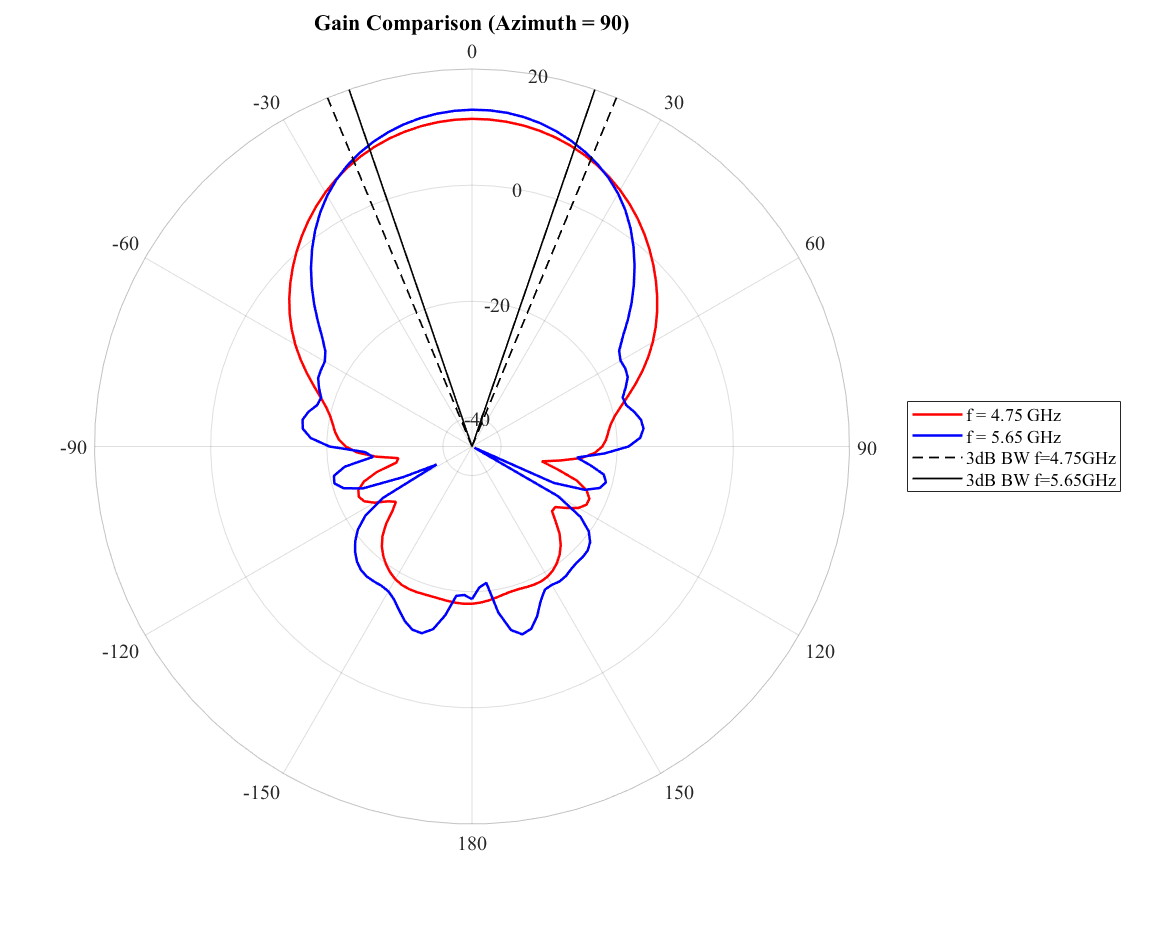
\includegraphics[width=1\textwidth]{figures/horn_elevation.png}
    \caption{Measured gain in the farfield at \SI{4.75}{\giga\hertz} and \SI{5.65}{\giga\hertz} (elevation plane).} 
    \label{fig:horn_elevation}
\end{figure}

The figure \ref{fig:horn_azimuth} below shows the azimuth plane of the horn antenna as measured in the anechoic chamber. The red line shows the gain for the antenna at $f=\SI{4.75}{\giga\hertz}$ and the blue line shows the gain for the antenna at $f=\SI{5.65}{\giga\hertz}$. The maximum gain is \SI{12.99}{\decibel} at \SI{0}{\degree}. 
\begin{figure}[H]
    \centering
    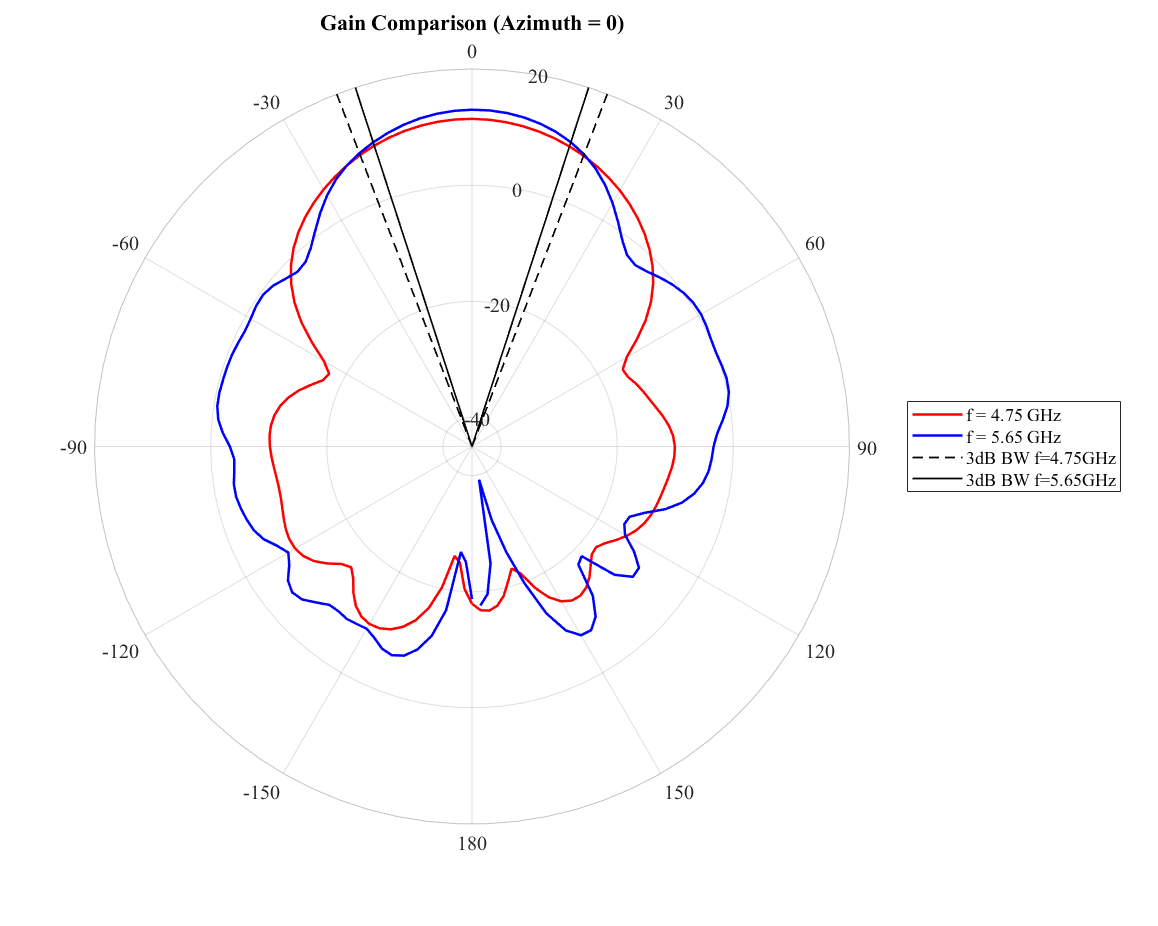
\includegraphics[width=1\textwidth]{figures/horn_azimuth.png}
    \caption{Measured gain in the farfield at \SI{4.75}{\giga\hertz} and \SI{5.65}{\giga\hertz} (azimuth plane).} 
    \label{fig:horn_azimuth}
\end{figure}

Simultaneously the maximum gain of the antenna over the frequency spectrum at any measured angle was measured as seen on the figure \ref{fig:gain_meas}. The measurement shows that the gain, generally, increases as the frequency increases.
\begin{figure}[H]
    \centering
    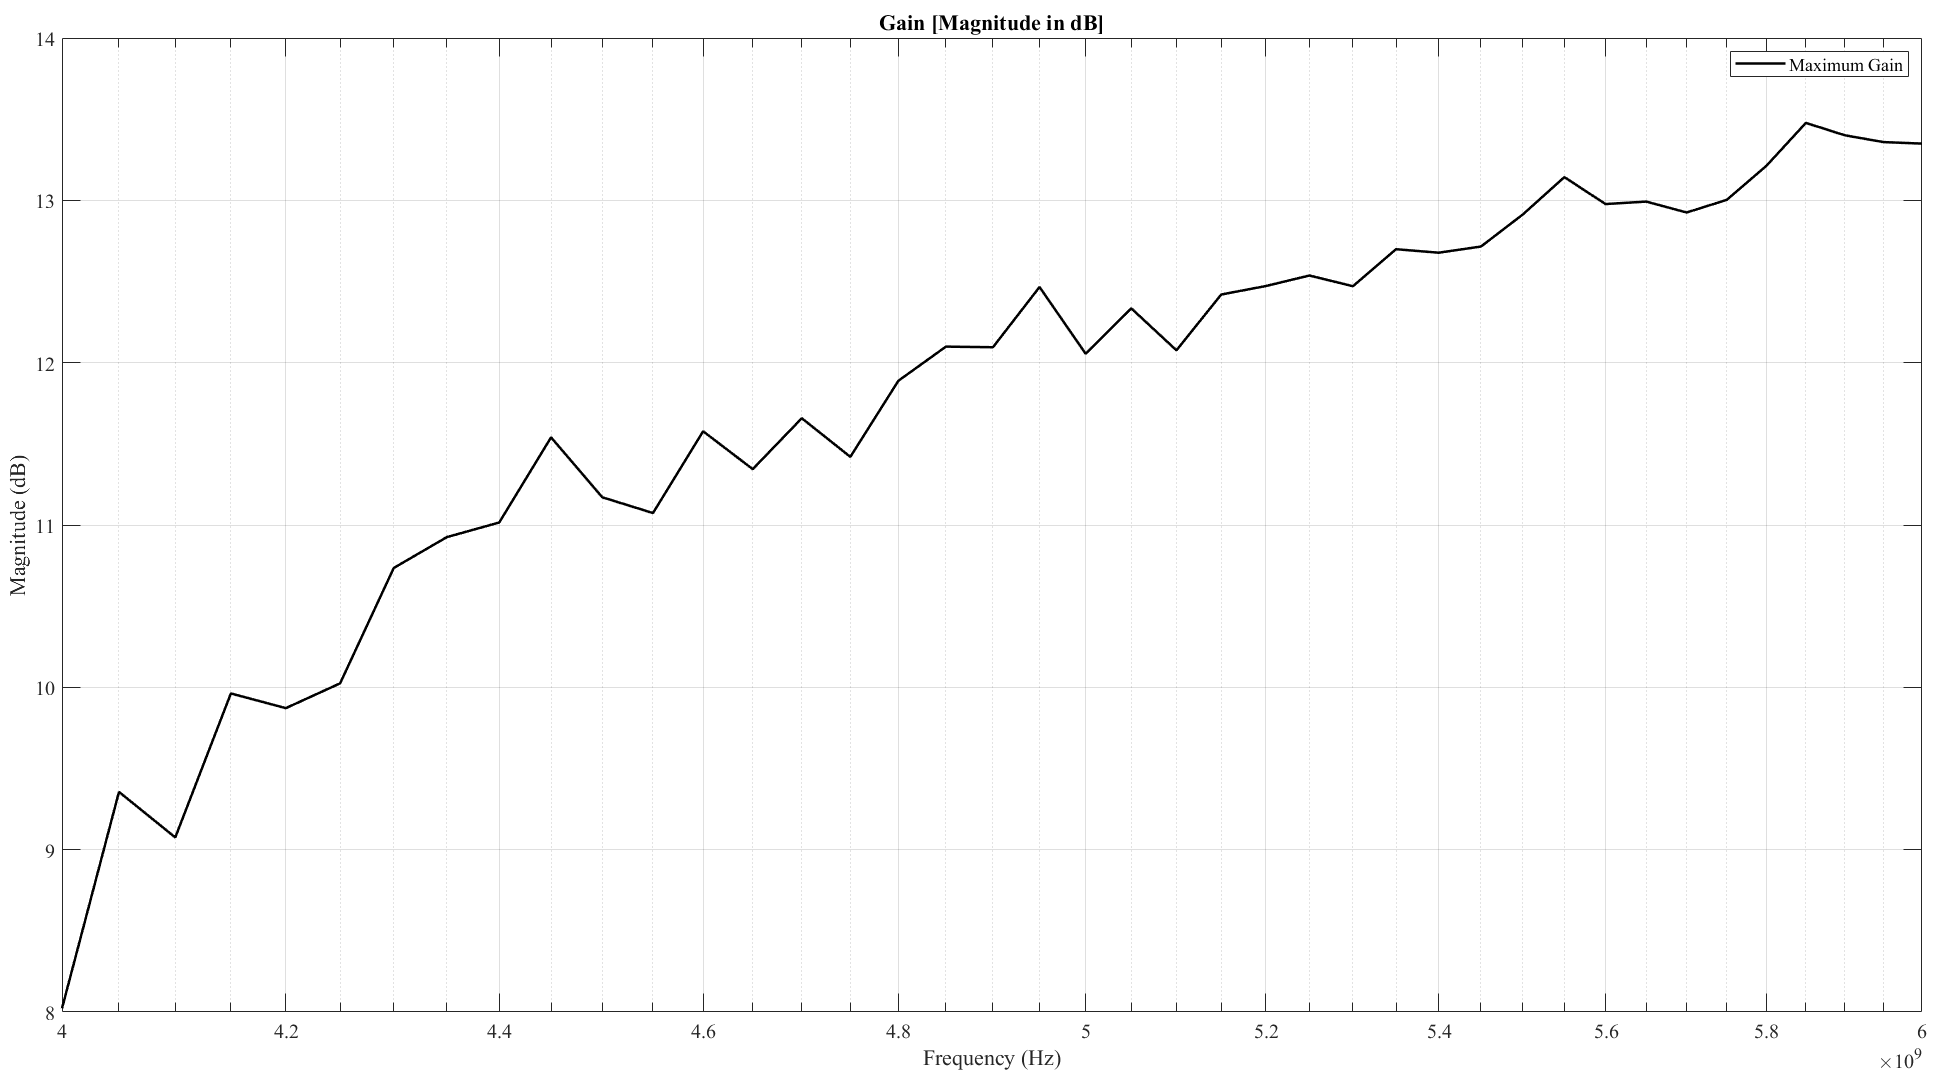
\includegraphics[width=1\textwidth]{figures/gain_meas.png}
    \caption{Measured maximum gain at any measured angle in the frequency spectrum from \SI{4}{\giga\hertz} to \SI{6}{\giga\hertz}.} \label{fig:gain_meas}
\end{figure}

\section{Accept Test} \label{s:accept_test}
The aim of this test is to test the full function of the developed product. The test must show that the receiver antenna on the turntable is able to scan the test area and measure the received power at fixed angles, before selection the location with the maximum received power and focusing its beam on that location. The test also contains test of intruder detection. In these scenarios the line-of-sight between the transmitter and receiver antennas is broken by an object. 

\subsubsection{Equipment}
To perform the test, the following equipment is needed:

\begin{itemize}
    \item HEAD Acoustics Remote-operated Turntable, model HRT I 6498, with \SI{24}{\volt} DC \SI{60}{W} power supply
    \item D-sub 9-pin to USB-A cable to connect turntable to PC
    \item PC with one USB-A port and one LAN port
    \item Rohde \& Schwarz ZVB 8 Vector Network Analyzer
    \item Network cable (8-pin RJ-45 connector) to connect VNA to PC
    \item Two identical horn antennas with dimensions as seen on figure \ref{fig:horn_design} in section \ref{s:ant_design}
    \item Two \SI{50}{\ohm} antenna cables
\end{itemize}

Moreover, the test must be performed in a controlled environment in order to ensure that the turntable and VNA can function optimally. The temperature must not be below \SI{5}{\celsius} or above \SI{40}{\celsius} with a relative humidity in the range \SI{20}{\percent} - \SI{80}{\percent}~\cite{hrt_i_data_sheet}\cite{vna_data_sheet_spec}.

\subsubsection{Procedure}
The following steps outline how to perform the test:

\begin{enumerate}
    \item Power ZVB8 and HRT I. 
    \item Calibrate ZVB8 with calibration unit.
    \item Connect Windows PC to ZVB8 and HRT I.
    \item Connect transmitter antenna to port 2 on ZVB8 with antenna cable. Set channel power level to \SI{10}{dBm}.
    \item Connect receiver antenna to port 1 on ZVB8 with antenna cable.
    \item Setup transmitter antenna to point towards receiver antenna creating a line-of-sight between the two antennas. 
    \item Mount the receiver antenna on HRT I.
    \item Load Python code on Windows PC and run control program.
\end{enumerate}

Repeat the test procedure for different setups; antennas pointing straight to each other with and without intruder person, with the antennas in either corner of a room with and without intruder table, and with the transmitter perpendicular to the receiver antenna. Figure \ref{fig:experiment-setup} shows a simple diagram of the test setup from a horizontal view.

\begin{figure}[H]
    \centering
    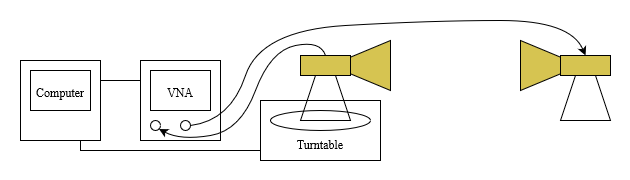
\includegraphics[width=0.8\textwidth]{figures/accept_test_setup.png}
    \caption{Setup for test of functionality of beam steering device.} \label{fig:experiment-setup}
\end{figure}

\subsubsection{Result}
As mentioned the test was performed with several setups. The tables in this section include a condensed version of the logs printed with every test of the full setup. The logs can be found through the link in appendix \ref{a:code}. 

The test scenario \textit{straight line-of-sight} is made with the antennas pointing directly towards each other. The distance between the antennas is $d=\SI{5.4}{\meter}$. The start position is \SI{10}{\degree}, the end position is \SI{150}{\degree} and the increase is \SI{20}{\degree}. The following figure \ref{fig:a2_1} shows the setup:
\begin{figure}[H]
    \centering
    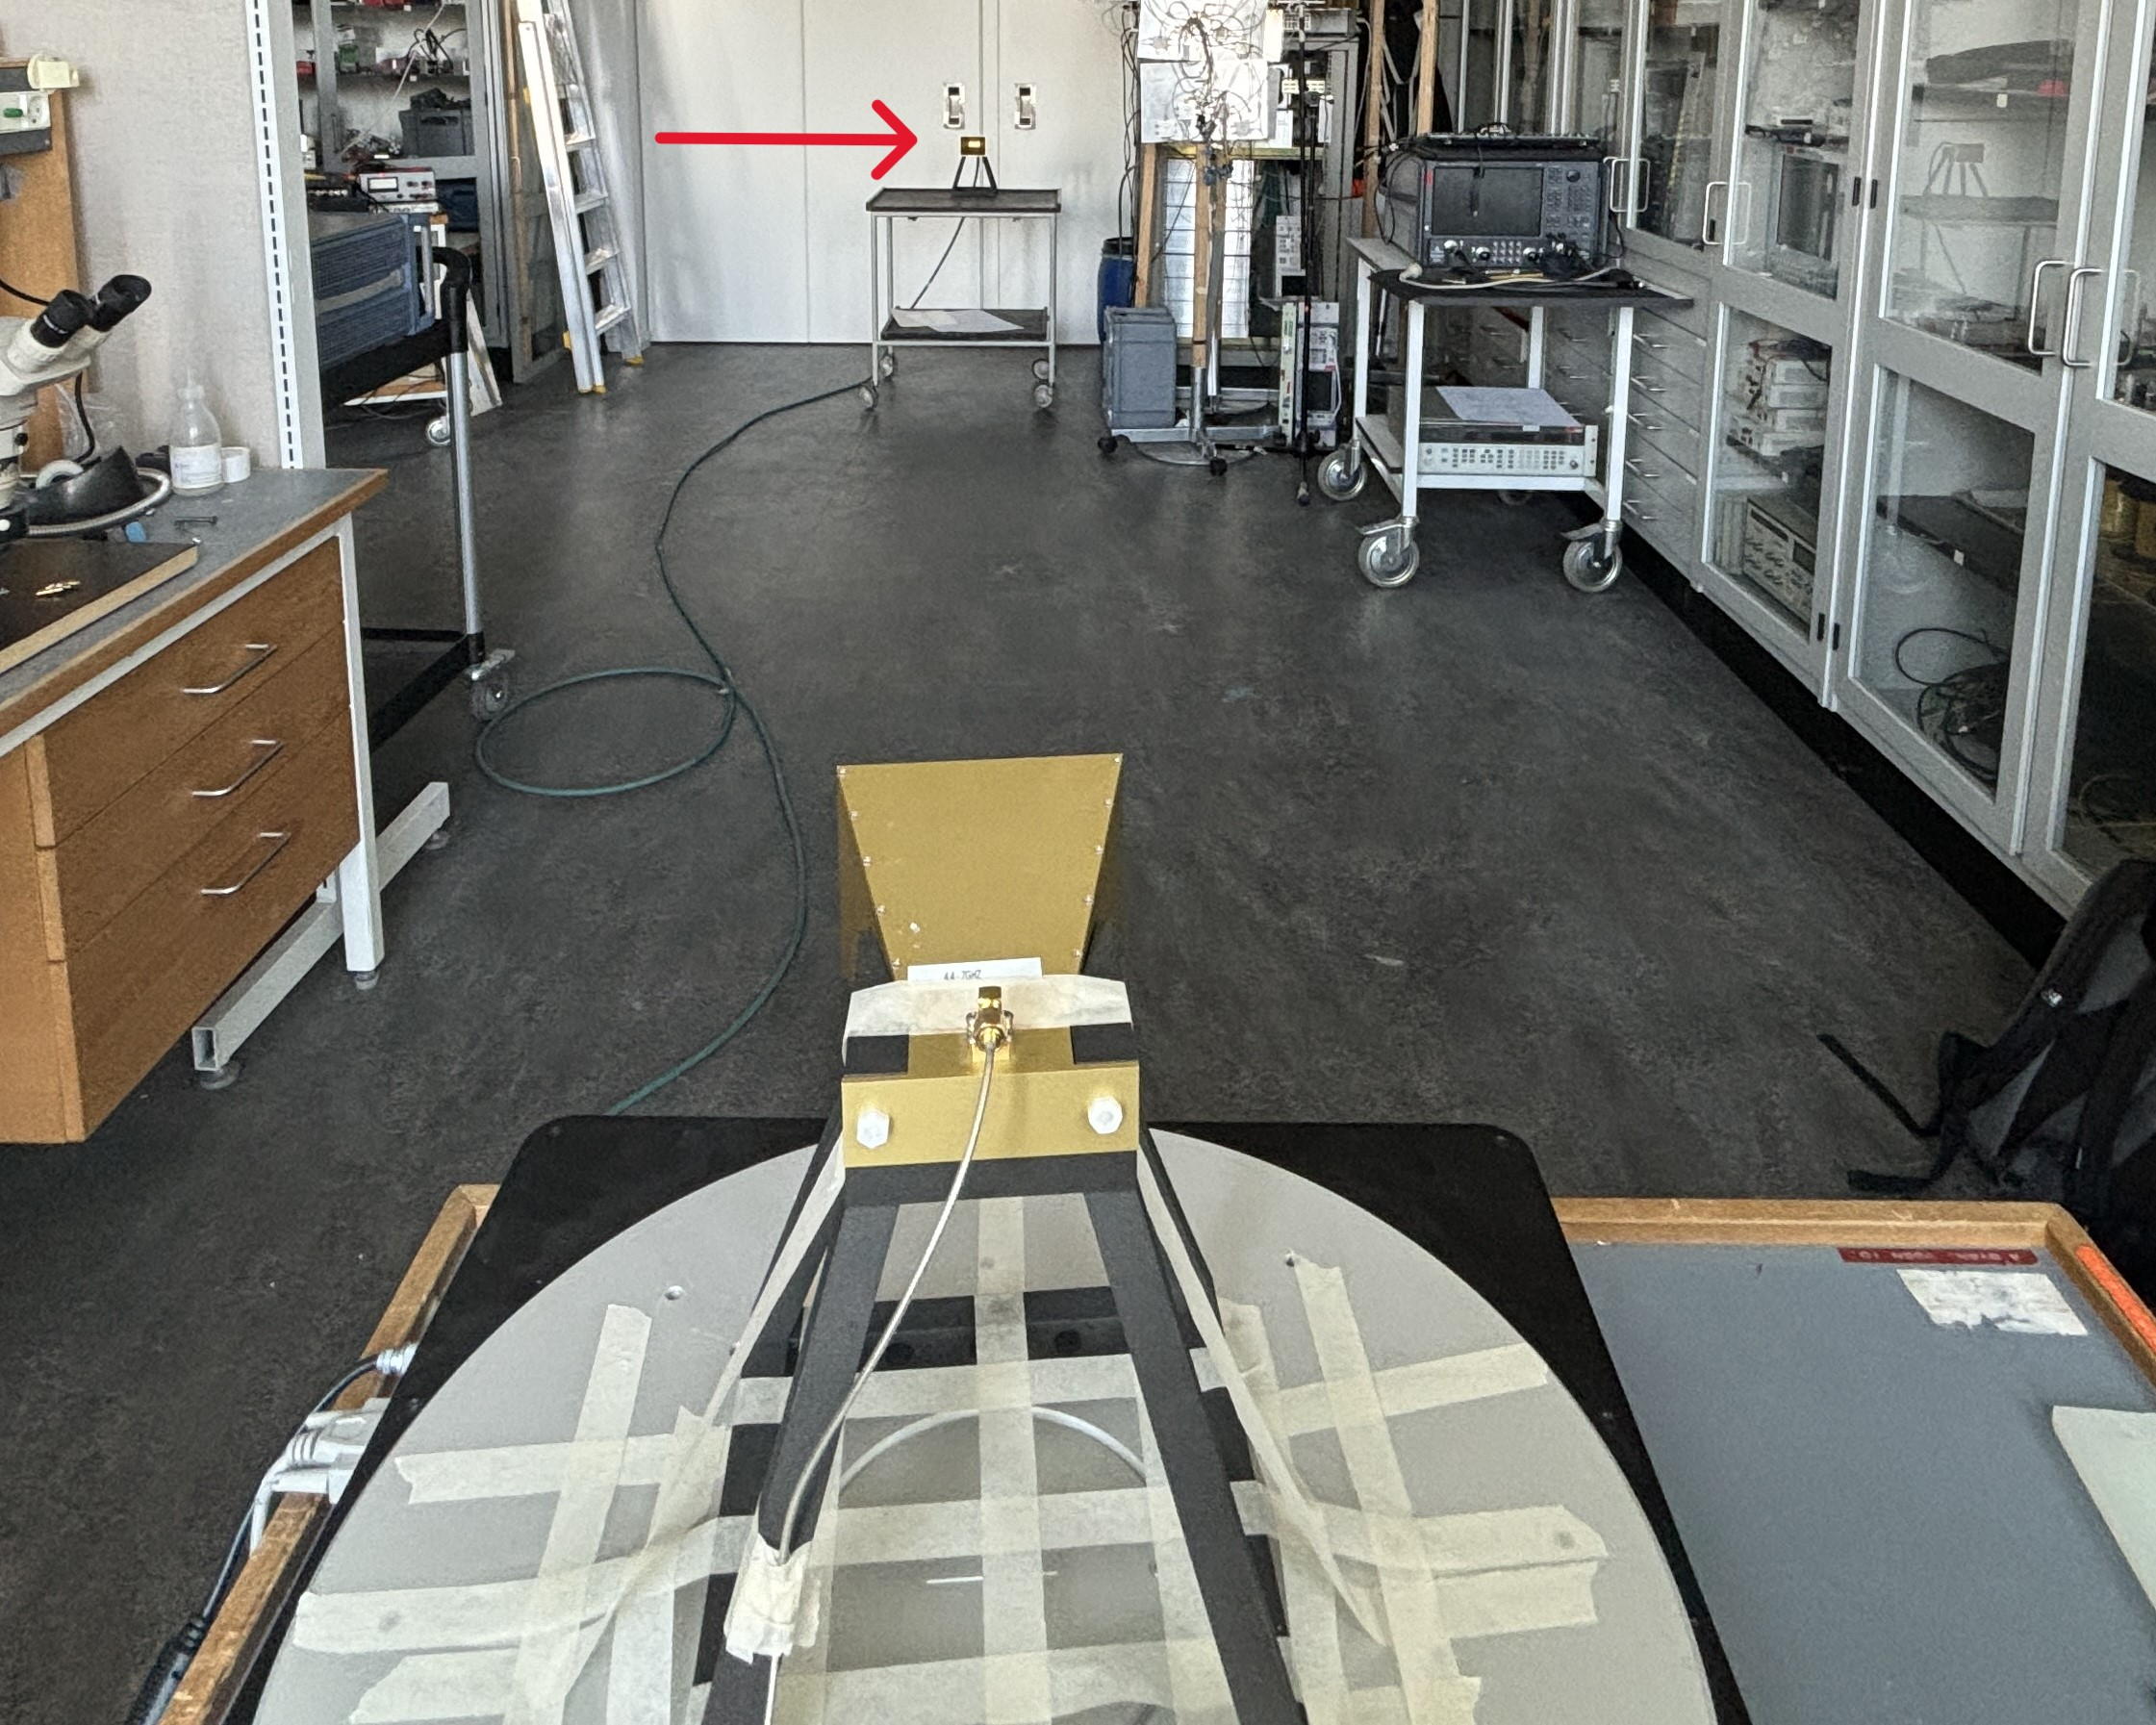
\includegraphics[width=0.7\textwidth]{figures/test_los_straight.JPG}
    \caption{View from receiver antenna at position \SI{50}{\degree} towards transmitter antenna.} \label{fig:a2_1}
\end{figure}

The test results can be found in table \ref{tab:a2_1a} and \ref{tab:a2_1b}.
\begin{table}[H]
    \centering
    \begin{tabular}{l|l|l|l}
        \multicolumn{4}{l}{\textbf{Frequency = 4.75 GHz}}         \\
        \hline
        \textbf{Position} & \multicolumn{3}{l}{\textbf{Power Measurement (dB)}} \\
        \textbf{(degrees)}  & Test 1    & Test 2  & Test 3  \\
        \hline
        \hline
        10      & -51.33    & -51.15    & -51.01 \\
        30      & \textcolor{red}{-46.82}    & \textcolor{red}{-46.63}    & \textcolor{red}{-46.52} \\
        50      & -46.96    & -46.77    & -46.66 \\
        70      & -49.07    & -48.88    & -48.78 \\
        90      & -55.30    & -55.18    & -48.78 \\
        110     & -70.33    & -69.99    & -69.81 \\
        130     & -67.82    & -67.30    & -67.27 \\
        150     & -66.85    & -66.73    & -66.58
        \end{tabular}
    \caption{Table of power measurements at each position repeated three times at frequency $f=\SI{4.75}{\giga\hertz}$. The maximum gain of each test is highlighted in red.}
    \label{tab:a2_1a}
\end{table}

\begin{table}[H]
    \centering
    \begin{tabular}{l|l|l|l}
        \multicolumn{4}{l}{\textbf{Frequency = 5.65 GHz}}         \\
        \hline
        \textbf{Position} & \multicolumn{3}{l}{\textbf{Power Measurement (dB)}} \\
        \textbf{(degrees)}  & Test 1    & Test 2  & Test 3  \\
        \hline
        \hline
        10      & -45.96    & -46.04    & -45.99 \\
        30      & -34.88    & -34.81    & -34.76 \\
        50      & \textcolor{red}{-31.05}    & \textcolor{red}{-30.99}    & \textcolor{red}{-30.93} \\
        70      & -34.61    & -34.56    & -34.51 \\
        90      & -49.59    & -49.54    & -49.47 \\
        110     & -64.89    & -64.79    & -64.67 \\
        130     & -50.16    & -50.15    & -50.15 \\
        150     & -58.68    & -58.68    & -58.79
        \end{tabular}
    \caption{Table of power measurements at each position repeated three times at frequency $f=\SI{5.65}{\giga\hertz}$. The maximum gain of each test is highlighted in red.}
    \label{tab:a2_1b}
\end{table}

Comparing the results of the direct, straight line-of-sight without intruder between $f=\SI{4.75}{\giga\hertz}$ and $f=\SI{5.65}{\giga\hertz}$ it is seen that the maximum gain is not at the same angle step but instead at \SI{30}{\degree} at $f=\SI{4.75}{\giga\hertz}$ and at \SI{50}{\degree} at $f=\SI{5.65}{\giga\hertz}$. Looking at the data for $f=\SI{4.75}{\giga\hertz}$, it can be seen that the difference in magnitude from \SI{30}{\degree} to \SI{50}{\degree} is very small (<\SI{0.14}{\decibel}) where its larger (>\SI{3.82}{\decibel}) for $f=\SI{5.65}{\giga\hertz}$ for the same angle step. This indicates that at $f=\SI{5.65}{\giga\hertz}$ the beam of the horn antenna is narrower. The gain is also larger at $f=\SI{5.65}{\giga\hertz}$ at averagely \SI{30.99}{\decibel} compared to the gain at $f=\SI{4.75}{\giga\hertz}$ at averagely \SI{-46.66}{\decibel}.

The test scenario \textit{straight with person intruder} is made with the antennas pointing directly towards each other. The distance between the antennas is $d=\SI{5.4}{\meter}$ and the object, the person, is placed \SI{2}{\meter} from the transmitter and \SI{3.4}{\meter} from the receiver. The start position is \SI{10}{\degree}, the end position is \SI{150}{\degree} and the increase is \SI{20}{\degree}. The following figure \ref{fig:a2_5} shows the setup:
\begin{figure}[H]
    \centering
    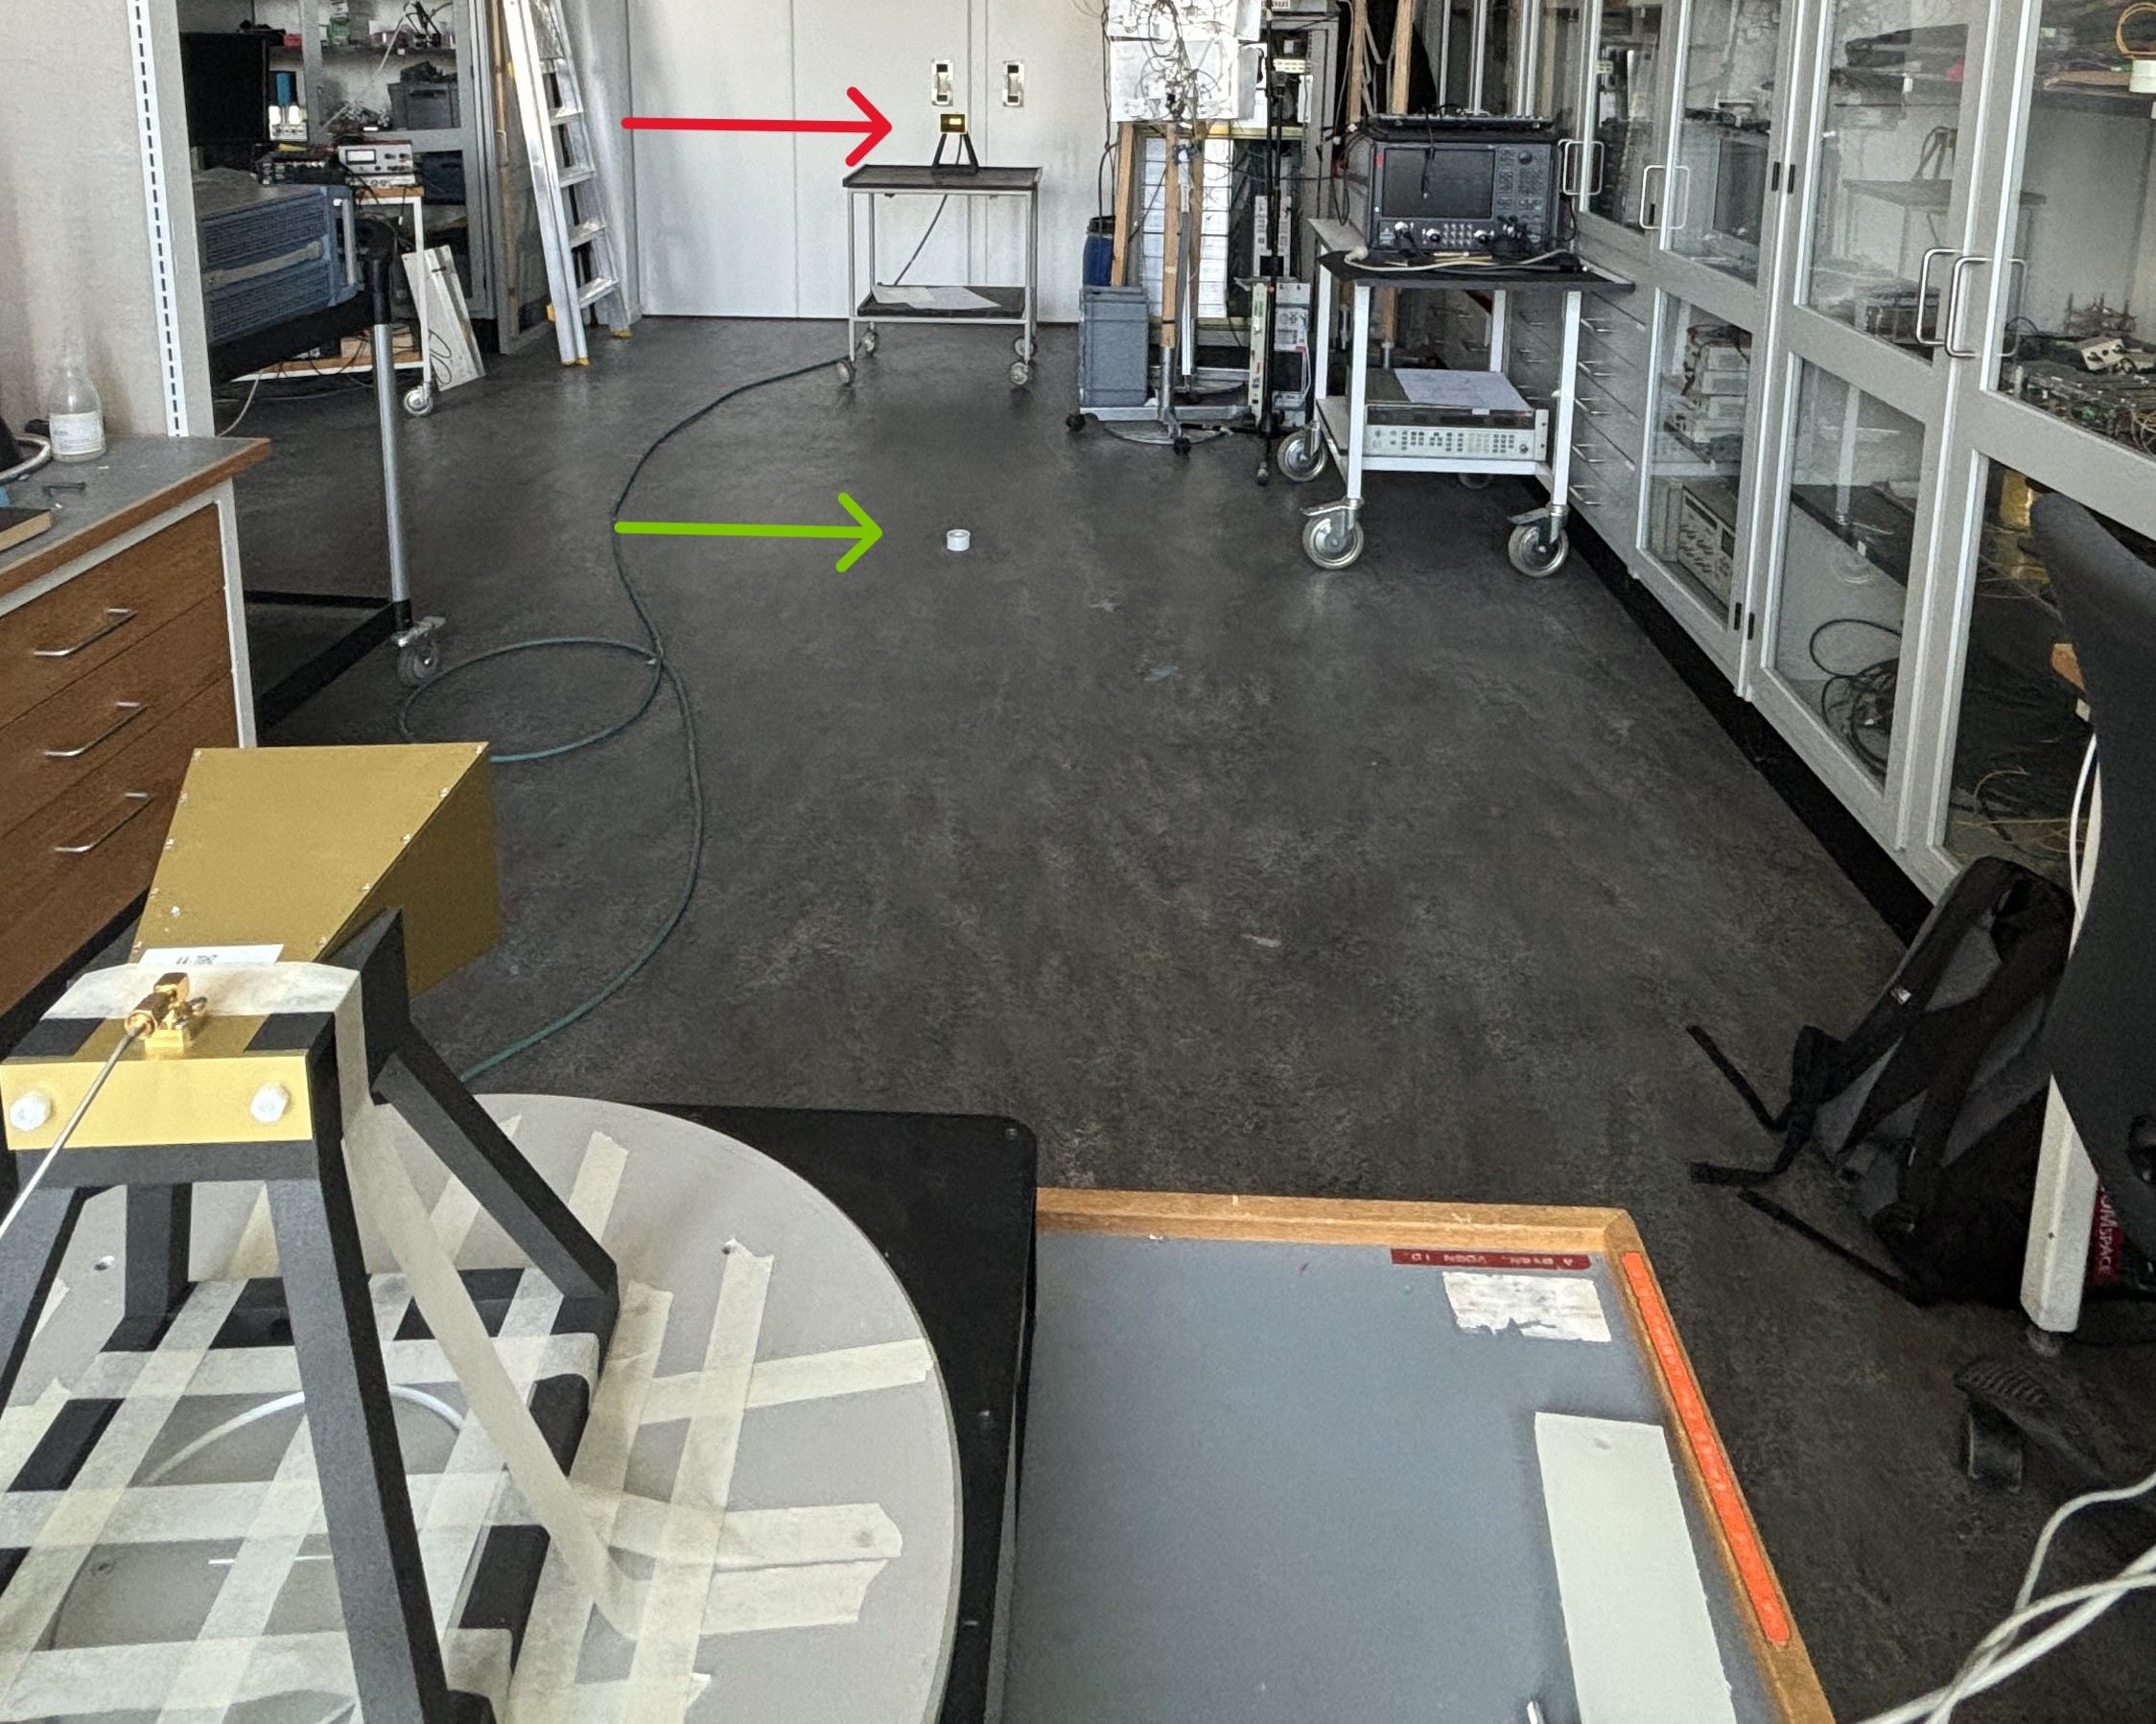
\includegraphics[width=0.7\textwidth]{figures/test_intruder_person.JPG}
    \caption{View from receiver antenna at position \SI{50}{\degree} towards transmitter antenna. The green arrow points towards the location on the where the person is.} \label{fig:a2_5}
\end{figure}

The test results can be found in table \ref{tab:a2_5a} and \ref{tab:a2_5b}.
\begin{table}[H]
    \centering
    \begin{tabular}{l|l|l|l}
        \multicolumn{4}{l}{\textbf{Frequency = 4.75 GHz}}         \\
        \hline
        \textbf{Position} & \multicolumn{3}{l}{\textbf{Power Measurement (dB)}} \\
        \textbf{(degrees)}  & Test 1    & Test 2  & Test 3  \\
        \hline
        \hline
        10      & \textcolor{red}{-53.88}    & \textcolor{red}{-51.03}    & \textcolor{red}{-53.15} \\
        30      & -65.65    & -62.04    & -58.07 \\
        50      & -60.18    & -60.21    & -63.31 \\
        70      & -60.91    & -61.45    & -63.88 \\
        90      & -68.03    & -64.38    & -67.73 \\
        110     & -78.76    & -67.41    & -85.01 \\
        130     & -68.04    & -86.78    & -72.53 \\
        150     & -65.90    & -66.63    & -64.46
        \end{tabular}
    \caption{Table of power measurements at each position repeated three times at frequency $f=\SI{4.75}{\giga\hertz}$. The maximum gain of each test is highlighted in red.}
    \label{tab:a2_5a}
\end{table}

\begin{table}[H]
    \centering
    \begin{tabular}{l|l|l|l}
        \multicolumn{4}{l}{\textbf{Frequency = 5.65 GHz}}         \\
        \hline
        \textbf{Position} & \multicolumn{3}{l}{\textbf{Power Measurement (dB)}} \\
        \textbf{(degrees)}  & Test 1    & Test 2  & Test 3  \\
        \hline
        \hline
        10      & -48.58    & \textcolor{red}{-44.45}    & -44.61 \\
        30      & -49.91    & -55.05    & -49.71 \\
        50      & \textcolor{red}{-43.50}    & -45.52    & \textcolor{red}{-39.29} \\
        70      & -44.11    & -45.39    & -40.85 \\
        90      & -54.07    & -62.36    & -50.56 \\
        110     & -63.50    & -74.10    & -59.50 \\
        130     & -52.11    & -53.01    & -52.56 \\
        150     & -60.54    & -57.75    & -58.38
        \end{tabular}
    \caption{Table of power measurements at each position repeated three times at frequency $f=\SI{5.65}{\giga\hertz}$. The maximum gain of each test is highlighted in red.}
    \label{tab:a2_5b}
\end{table}

The intruder changes the ability of the control program to correctly identify the direction of the transmitter antenna. At $f=\SI{4.75}{\giga\hertz}$ the maximum gain is at \SI{10}{\degree} which is in the direction of the close wall on the right-hand side when facing the transmitter. This indicates that the transmitter antenna propagates in the direction of the wall surface, so that the reflection is received at the receiver antenna. Further, the test data (seen in table \ref{tab:a2_5a}) also show that the gain at \SI{50}{\degree} and \SI{70}{\degree} is averagely higher than at other angle steps, indicating that the receiver antenna still can detect the transmitter with a person intruder, but that the intruder does affect the received signal. At $f=\SI{5.65}{\giga\hertz}$ the data is not consistent across all three tests. The receiver antenna receives the maximum gain in the same direction as the transmitter antenna, which is evident when comparing to the same setup without intruder, where the maximum gain is also at \SI{50}{\degree}, meaning that it is not possible to detect the intruder when only looking at the direction of the maximum gain at $f=\SI{5.65}{\giga\hertz}$. However, comparing the values, the gain measured with an intruder is averagely $\SI{42.41}{\decibel}-\SI{30.99}{\decibel}=\SI{11.42}{\decibel}$ less than without intruder. 

The test scenario \textit{corner-to-corner line-of-sight} is made with the antennas pointing directly towards each other from a skew angle in each their own corner of the room. The distance between the antennas is not measured. The start position is \SI{10}{\degree}, the end position is \SI{150}{\degree} and the increase is \SI{20}{\degree}. The following figure \ref{fig:a2_2} shows the setup:
\begin{figure}[H]
    \centering
    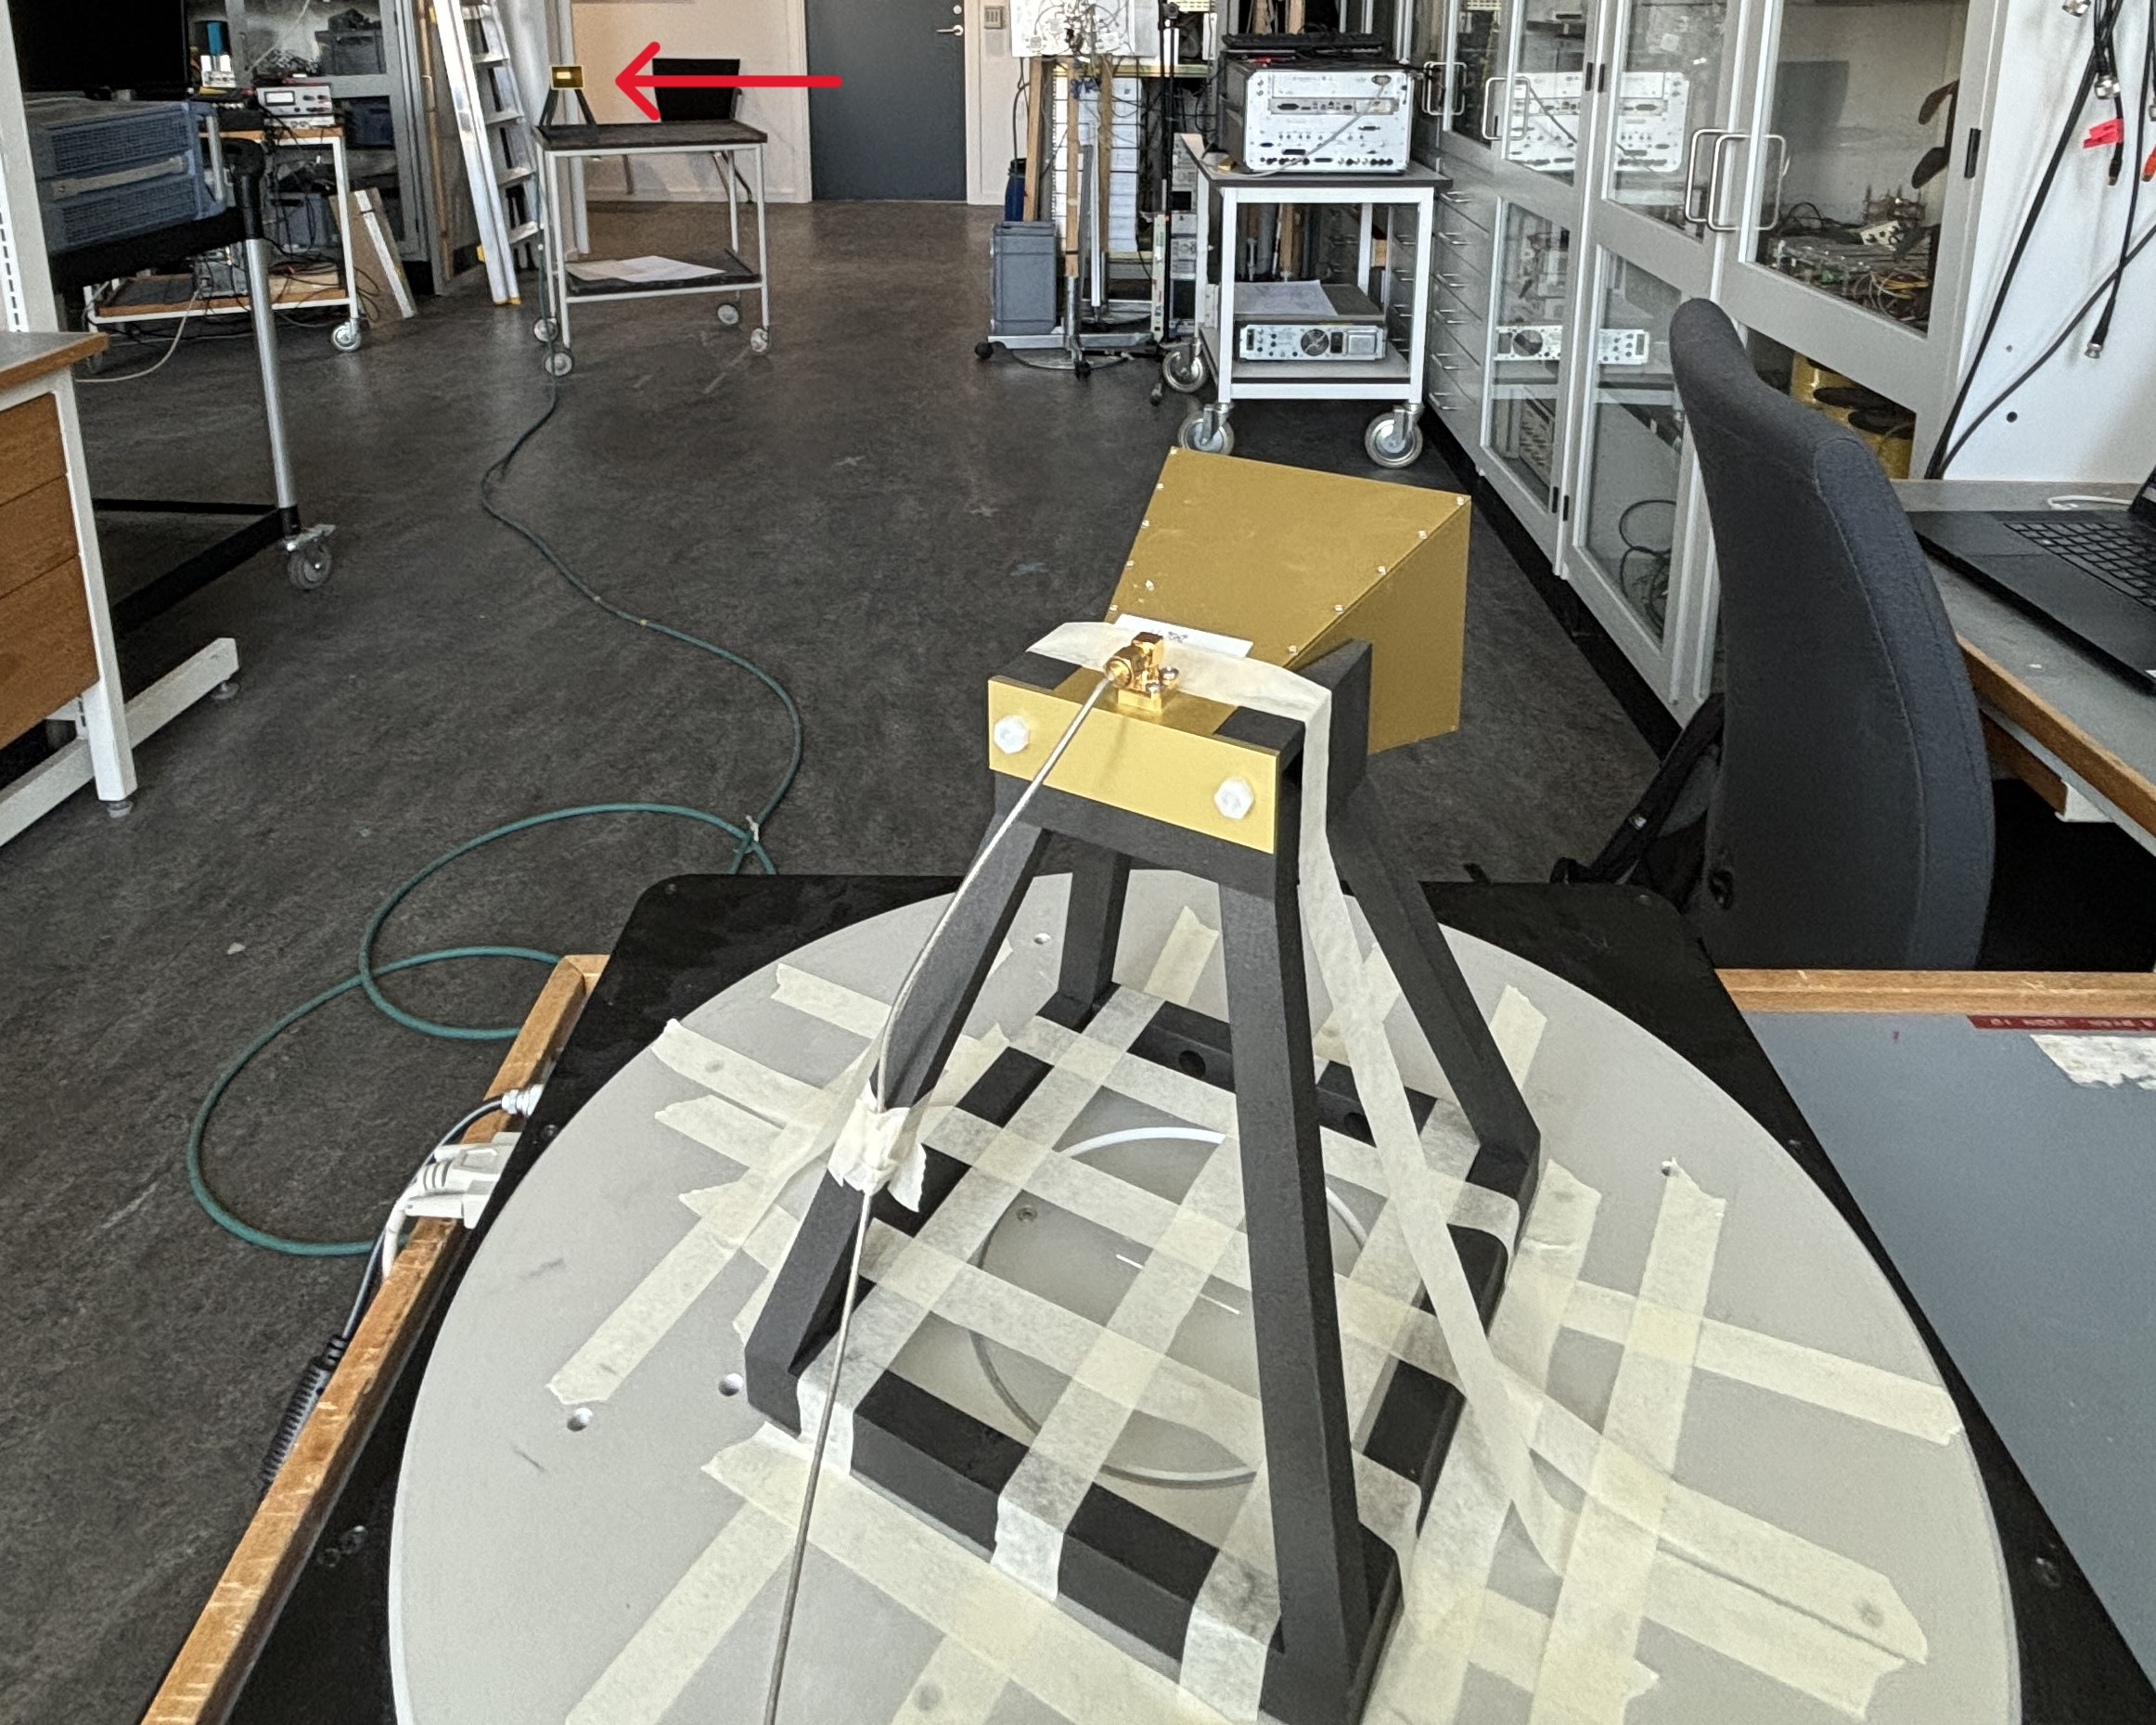
\includegraphics[width=0.7\textwidth]{figures/test_los_corner.JPG}
    \caption{View from receiver antenna at position \SI{10}{\degree} towards transmitter antenna.} \label{fig:a2_2}
\end{figure}

The test results can be found in table \ref{tab:a2_2a} and \ref{tab:a2_2b}.
\begin{table}[H]
    \centering
    \begin{tabular}{l|l|l|l}
        \multicolumn{4}{l}{\textbf{Frequency = 4.75 GHz}}         \\
        \hline
        \textbf{Position} & \multicolumn{3}{l}{\textbf{Power Measurement (dB)}} \\
        \textbf{(degrees)}  & Test 1    & Test 2  & Test 3  \\
        \hline
        \hline
        10      & -59.79    & -59.20    & -59.13 \\
        30      & -52.45    & -52.08    & -52.00 \\
        50      & -53.22    & -52.94    & -52.86 \\
        70      & \textcolor{red}{-48.34}    & \textcolor{red}{-48.11}    & \textcolor{red}{-48.06} \\
        90      & -51.32    & -51.09    & -51.04 \\
        110     & -70.33    & -58.41    & -58.33 \\
        130     & -75.39    & -75.27    & -75.29 \\
        150     & -62.40    & -62.15    & -62.07
        \end{tabular}
    \caption{Table of power measurements at each position repeated three times at frequency $f=\SI{4.75}{\giga\hertz}$. The maximum gain of each test is highlighted in red.}
    \label{tab:a2_2a}
\end{table}

\begin{table}[H]
    \centering
    \begin{tabular}{l|l|l|l}
        \multicolumn{4}{l}{\textbf{Frequency = 5.65 GHz}}         \\
        \hline
        \textbf{Position} & \multicolumn{3}{l}{\textbf{Power Measurement (dB)}} \\
        \textbf{(degrees)}  & Test 1    & Test 2  & Test 3  \\
        \hline
        \hline
        10      & -45.73    & -45.41    & -45.37 \\
        30      & -43.94    & -43.82    & -43.79 \\
        50      & -34.21    & -34.01    & -33.96 \\
        70      & \textcolor{red}{-32.29}    & \textcolor{red}{-32.15}    & \textcolor{red}{-32.10} \\
        90      & -37.35    & -37.27    & -37.23 \\
        110     & -51.65    & -51.62    & -51.63 \\
        130     & -68.07    & -68.20    & -68.02 \\
        150     & -56.72    & -56.73    & -56.66
        \end{tabular}
    \caption{Table of power measurements at each position repeated three times at frequency $f=\SI{5.65}{\giga\hertz}$. The maximum gain of each test is highlighted in red.}
    \label{tab:a2_2b}
\end{table}

The test scenario \textit{corner-to-corner with table intruder} is made with the transmitting antenna pointing in the direction of the receiver antenna, with the antennas each in an opposite corner. The distance between the antennas is not measured. The start position is \SI{10}{\degree}, the end position is \SI{150}{\degree} and the increase is \SI{20}{\degree}. The following figure \ref{fig:a2_4} shows the setup:
\begin{figure}[H]
    \centering
    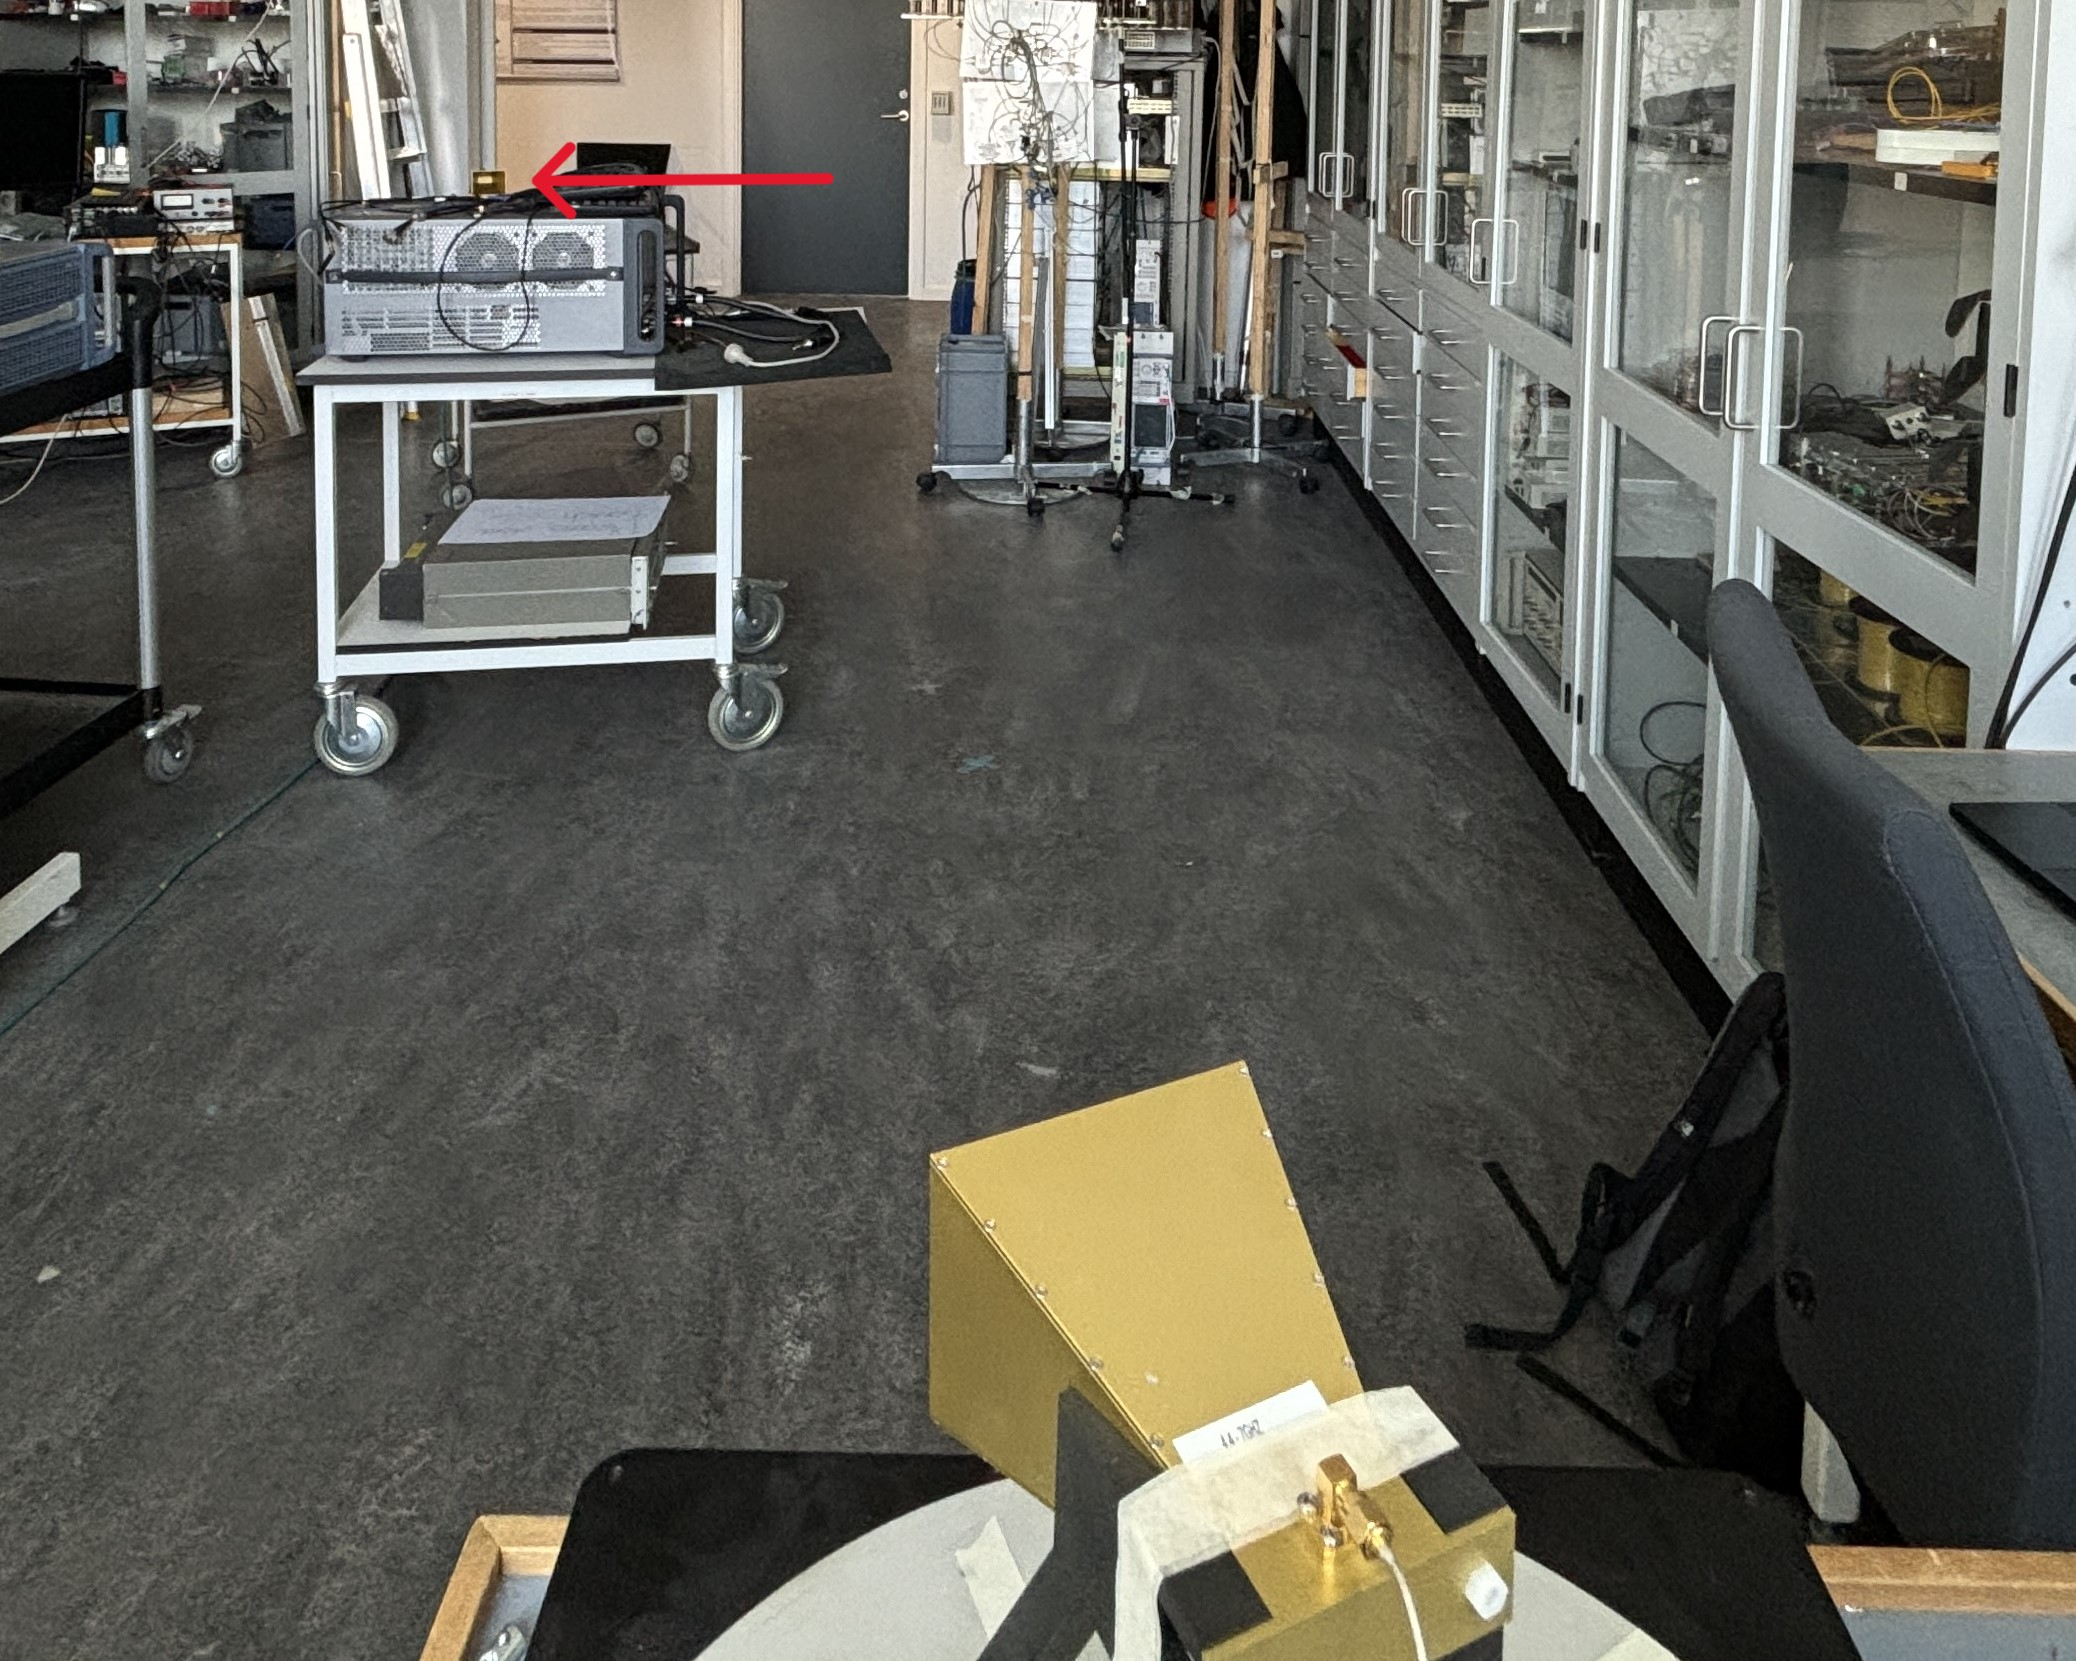
\includegraphics[width=0.7\textwidth]{figures/test_intruder_table.JPG}
    \caption{View from receiver antenna at position \SI{70}{\degree} towards transmitter antenna.} \label{fig:a2_4}
\end{figure}

The test results can be found in table \ref{tab:a2_4a} and \ref{tab:a2_4b}.
\begin{table}[H]
    \centering
    \begin{tabular}{l|l|l|l}
        \multicolumn{4}{l}{\textbf{Frequency = 4.75 GHz}}         \\
        \hline
        \textbf{Position} & \multicolumn{3}{l}{\textbf{Power Measurement (dB)}} \\
        \textbf{(degrees)}  & Test 1    & Test 2  & Test 3  \\
        \hline
        \hline
        10      & \textcolor{red}{-57.75}    & \textcolor{red}{-57.52}    & \textcolor{red}{-57.40} \\
        30      & -59.87    & -59.68    & -59.57 \\
        50      & -65.42    & -65.22    & -65.14 \\
        70      & -62.53    & -62.40    & -62.26 \\
        90      & -59.81    & -59.60    & -59.49 \\
        110     & -64.94    & -64.81    & -64.74 \\
        130     & -68.94    & -68.80    & -68.63 \\
        150     & -62.11    & -61.96    & -61.85
        \end{tabular}
    \caption{Table of power measurements at each position repeated three times at frequency $f=\SI{4.75}{\giga\hertz}$. The maximum gain of each test is highlighted in red.}
    \label{tab:a2_4a}
\end{table}

\begin{table}[H]
    \centering
    \begin{tabular}{l|l|l|l}
        \multicolumn{4}{l}{\textbf{Frequency = 5.65 GHz}}         \\
        \hline
        \textbf{Position} & \multicolumn{3}{l}{\textbf{Power Measurement (dB)}} \\
        \textbf{(degrees)}  & Test 1    & Test 2  & Test 3  \\
        \hline
        \hline
        10      & -42.72    & -42.68    & -42.61 \\
        30      & -47.23    & -47.15    & -47.10 \\
        50      & \textcolor{red}{-35.61}    & \textcolor{red}{-35.55}    & \textcolor{red}{-35.49} \\
        70      & -35.83    & -35.75    & -35.69 \\
        90      & -41.75    & -41.68    & -41.61 \\
        110     & -54.32    & -54.25    & -54.20 \\
        130     & -77.38    & -76.43    & -76.11 \\
        150     & -57.60    & -57.49    & -57.27
        \end{tabular}
    \caption{Table of power measurements at each position repeated three times at frequency $f=\SI{5.65}{\giga\hertz}$. The maximum gain of each test is highlighted in red.}
    \label{tab:a2_4b}
\end{table}

Secondly, the test data shows the gain when the antennas are placed further apart in a corner-to-corner configuration with and without a table with a large, square electronic box as intruder. As seen on figure \ref{fig:a2_2} the transmitter antenna is moved to the left, meaning that the turntable must turn further in order to face the receiver antenna towards the transmitter antenna. This reflects in the results in table \ref{tab:a2_2a} and \ref{tab:a2_2b} where both at $f=\SI{4.75}{\giga\hertz}$ and $f=\SI{5.65}{\giga\hertz}$ the maximum gain is at \SI{70}{\degree}. Similarly as with the straight line-of-sight setup (seen in figure \ref{fig:a2_4}) the gain is larger at the higher frequency. The test is performed again with a table as an intruder. At $f=\SI{4.75}{\giga\hertz}$ the maximum gain is at position \SI{10}{\degree} which is not in the direction of the transmitting antenna but rather towards the right-hand wall when viewing from the receiver into the measurement space. This indicates that the receiver antenna receives reflections from the wall surface rather than directly from the transmitter. At $f=\SI{5.65}{\giga\hertz}$ this changes however, and the maximum gain is averagely \SI{35.55}{\decibel} at position \SI{50}{\degree}. The gain is approximately the same at position \SI{70}{\degree} as at position \SI{50}{\degree} with averagely difference of \SI{0.21}{\decibel}, which is the direction of the transmitter antenna. This indicates that even with an intruder, the receiver is able to locate the transmitter when at the frequency $f=\SI{5.65}{\giga\hertz}$. Comparing with the test without intruder, it can be seen at \SI{70}{\degree} there is a significant difference in what is measured in both tests and a comparable result at \SI{50}{\degree}. This indicates that the table intruder dampens the signal at \SI{70}{\degree} exactly and that the intruder can be detected when comparing the two tests.

The test scenario with \textit{antennas perpendicular to each other} is made with the transmitting antenna pointing perpendicular to the receiver antenna. The distance between the antennas is $d=\SI{5.4}{\meter}$. The start position is \SI{10}{\degree}, the end position is \SI{150}{\degree} and the increase is \SI{20}{\degree}. The following figure \ref{fig:a2_3} shows the setup:
\begin{figure}[H]
    \centering
    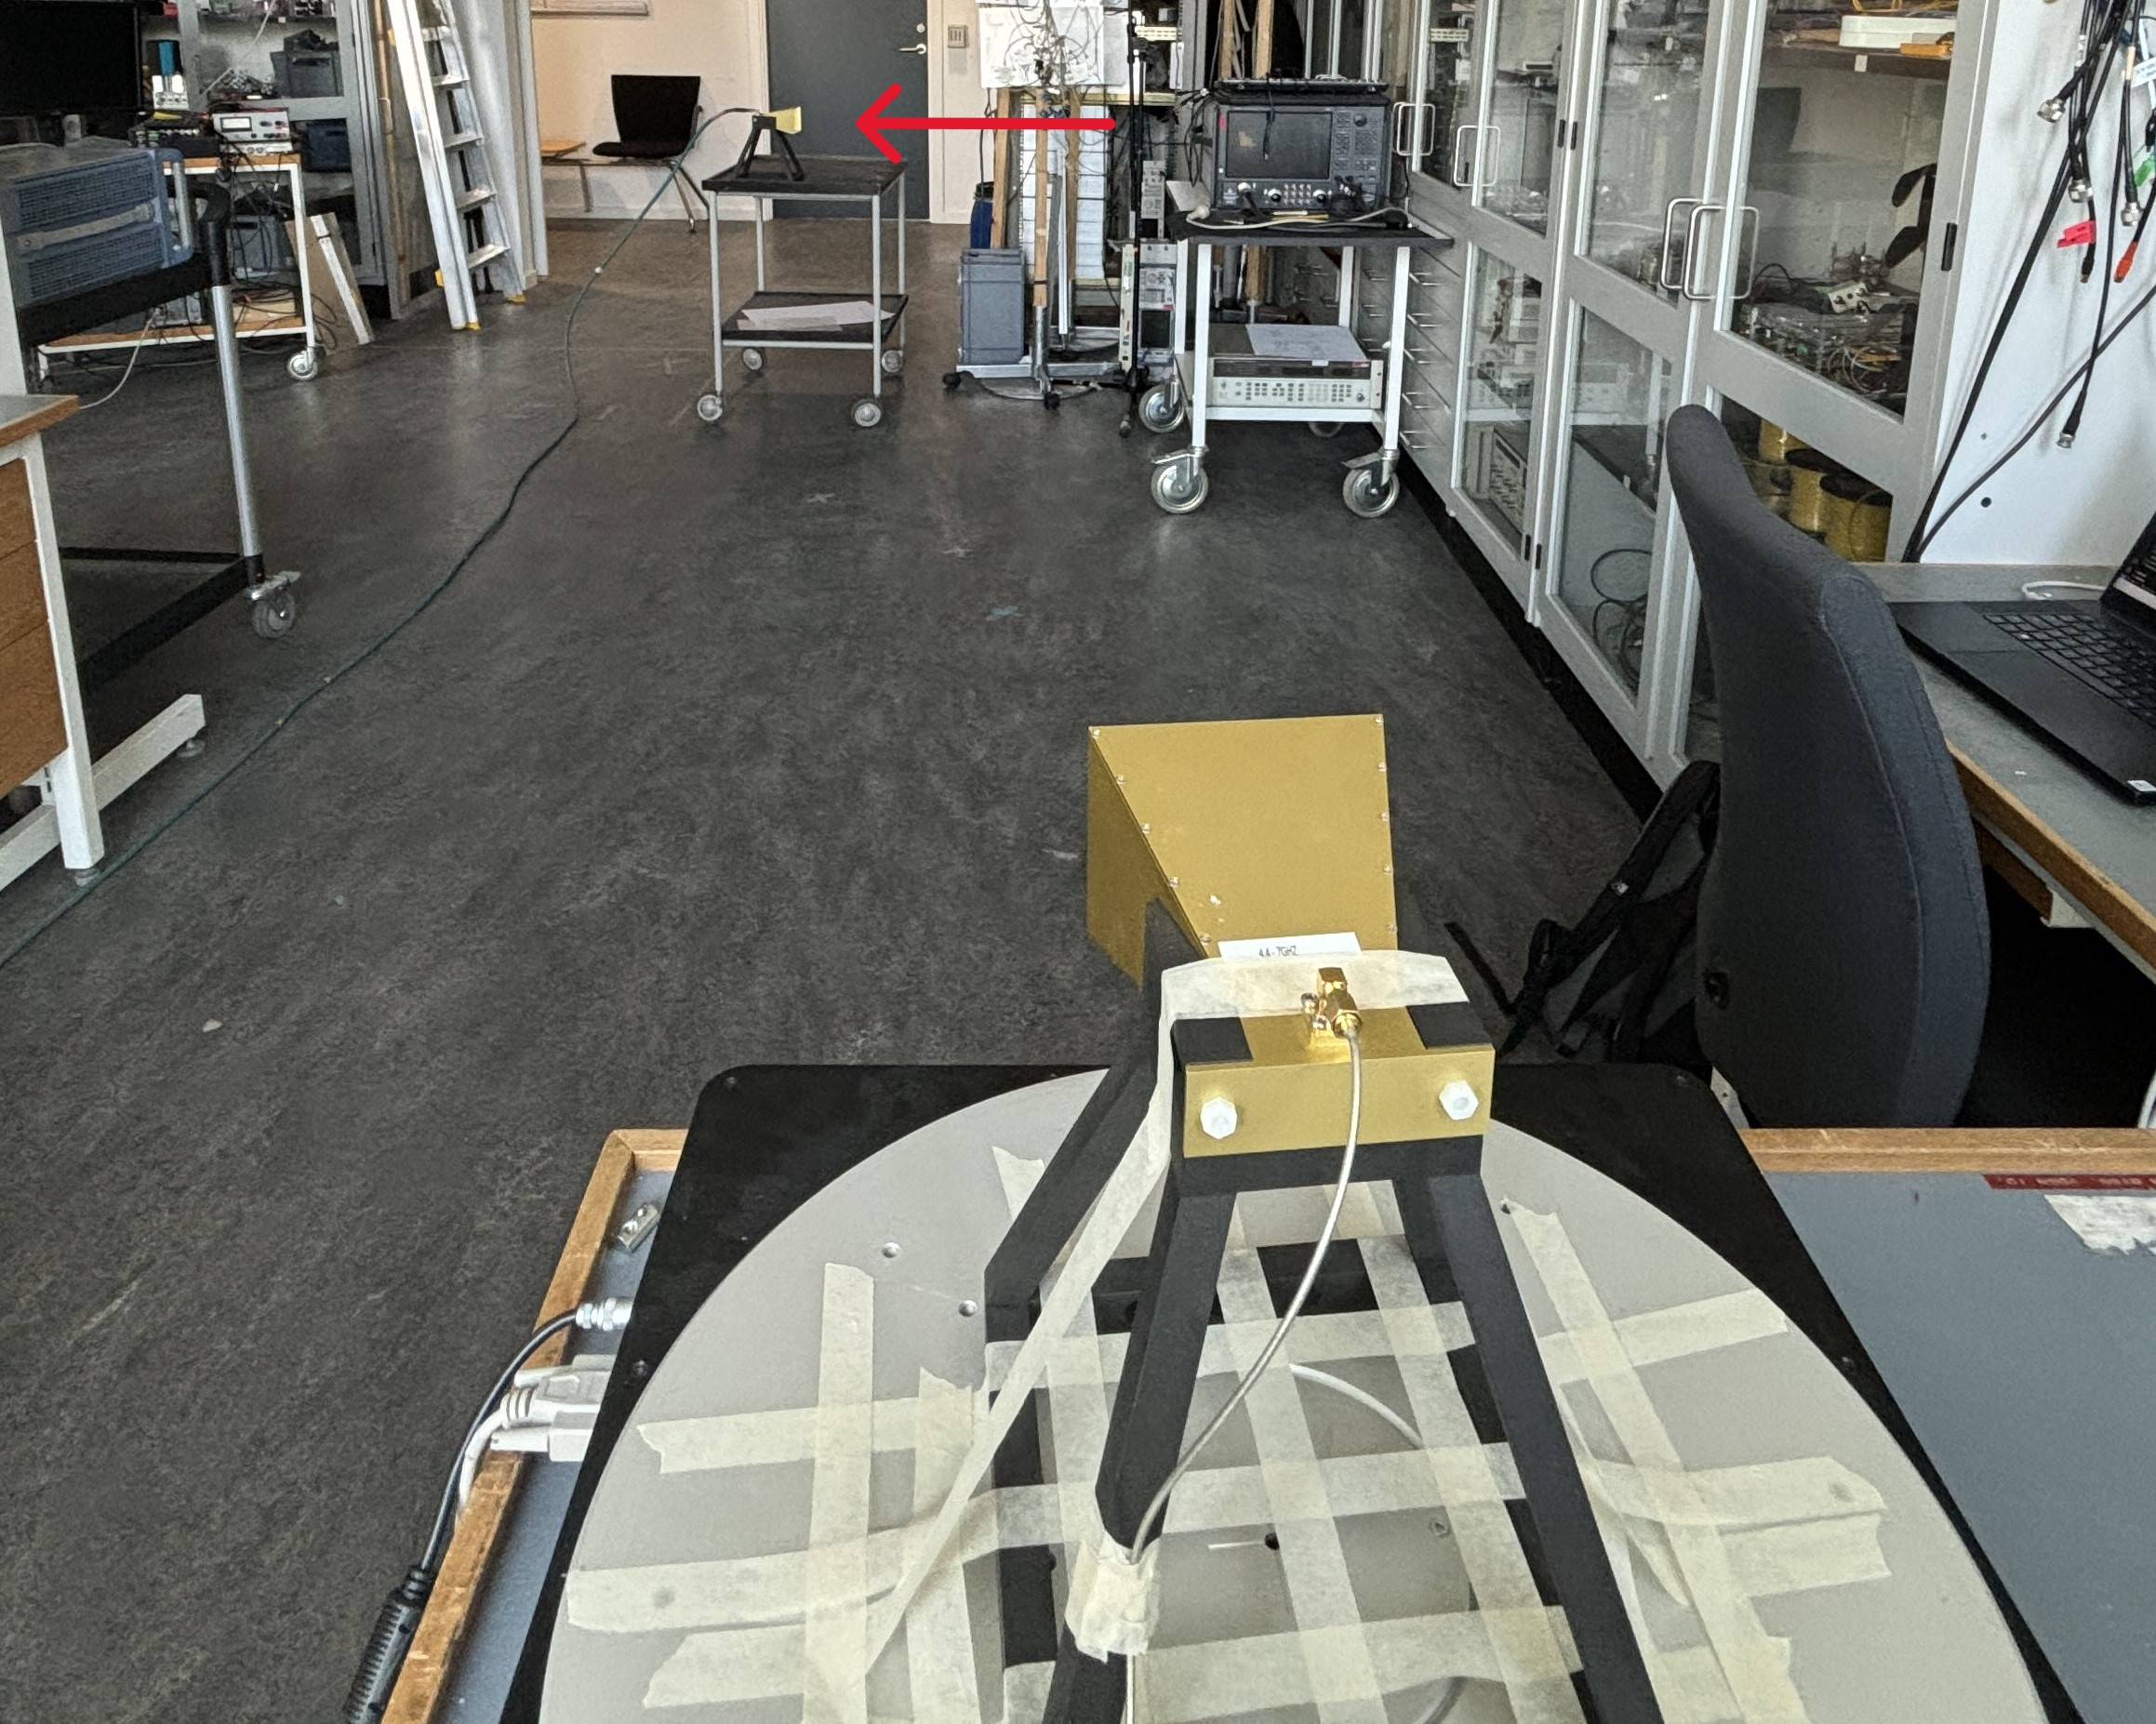
\includegraphics[width=0.7\textwidth]{figures/test_los_perpendicular.JPG}
    \caption{View from receiver antenna at position \SI{50}{\degree} towards transmitter antenna.} \label{fig:a2_3}
\end{figure}

The test results can be found in table \ref{tab:a2_3a} and \ref{tab:a2_3b}.
\begin{table}[H]
    \centering
    \begin{tabular}{l|l|l|l}
        \multicolumn{4}{l}{\textbf{Frequency = 4.75 GHz}}         \\
        \hline
        \textbf{Position} & \multicolumn{3}{l}{\textbf{Power Measurement (dB)}} \\
        \textbf{(degrees)}  & Test 1    & Test 2  & Test 3  \\
        \hline
        \hline
        10      & -74.27    & -74.29    & -74.33 \\
        30      & -72.12    & -72.13    & -72.21 \\
        50      & -77.03    & -76.04    & -75.61 \\
        70      & -71.35    & -71.17    & -70.58 \\
        90      & -69.45    & -69.47    & -69.71 \\
        110     & \textcolor{red}{-68.42}    & \textcolor{red}{-68.28}    & \textcolor{red}{-68.15} \\
        130     & -79.83    & -80.25    & -79.30 \\
        150     & -75.04    & -75.25    & -75.23
        \end{tabular}
    \caption{Table of power measurements at each position repeated three times at frequency $f=\SI{4.75}{\giga\hertz}$. The maximum gain of each test is highlighted in red.}
    \label{tab:a2_3a}
\end{table}

\begin{table}[H]
    \centering
    \begin{tabular}{l|l|l|l}
        \multicolumn{4}{l}{\textbf{Frequency = 5.65 GHz}}         \\
        \hline
        \textbf{Position} & \multicolumn{3}{l}{\textbf{Power Measurement (dB)}} \\
        \textbf{(degrees)}  & Test 1    & Test 2  & Test 3  \\
        \hline
        \hline
        10      & -58.25    & -58.25    & -58.34 \\
        30      & -55.13    & -55.12    & -54.97 \\
        50      & \textcolor{red}{-49.13}    & \textcolor{red}{-49.11}    & \textcolor{red}{-49.08} \\
        70      & -52.44    & -52.40    & -52.43 \\
        90      & -50.17    & -50.10    & -50.10 \\
        110     & -49.77    & -49.73    & -49.81 \\
        130     & -52.26    & -52.20    & -52.26 \\
        150     & -58.72    & -59.04    & -58.64
        \end{tabular}
    \caption{Table of power measurements at each position repeated three times at frequency $f=\SI{5.65}{\giga\hertz}$. The maximum gain of each test is highlighted in red.}
    \label{tab:a2_3b}
\end{table}

Finally, the transmitter antenna is placed perpendicular to the receiver facing the right-hand wall when looking from the receiver to the transmitter in a straight line-of-sight. The setup can be seen in figure \ref{fig:a2_3}. At $f=\SI{4.75}{\giga\hertz}$ the angle step with maximum gain is \SI{110}{\degree} which is not in the direction of the transmitter but instead in the opposite direction where the receiver antenna faces tables with test equipment. This shows that the receiver antenna is completely unable to detect the transmitter at $f=\SI{4.75}{\giga\hertz}$ if the transmitter is facing perpendicular to the the receiver antenna position. At $f=\SI{5.65}{\giga\hertz}$ the receiver antenna correctly identifies the transmitter to be at angle step \SI{50}{\degree}. This indicates that at $f=\SI{5.65}{\giga\hertz}$ the gain of the transmitter antenna at the $\theta=\SI{90}{\degree}$ angle in the azimuth plane is so large, that the receiver still detects the signal instead of reflections from objects in the measurement space. Comparing the average gain at the maximum (\SI{49.11}{\decibel}) to the gain at the same angle step as the maximum of $f=\SI{4.75}{\giga\hertz}$, which is \SI{110}{\degree}, at \SI{49.77}{\decibel}, it is clear that there is not a large difference. This indicates that the reflection measured at \SI{110}{\degree} seen both at $f=\SI{4.75}{\giga\hertz}$ and $f=\SI{5.65}{\giga\hertz}$ are significant to the result at both frequencies.

A further analysis of the test data can be made by comparing the measured gain at each position for all scenarios except the perpendicular setup. The data is plotted in figure \ref{fig:gain_vs_pos_475} for $f=\SI{4.75}{\giga\hertz}$ and in figure \ref{fig:gain_vs_pos_565} for $f=\SI{5.65}{\giga\hertz}$. At $f=\SI{4.75}{\giga\hertz}$ the graph shows that the intruder clearly dampens the received signal in both scenarios. The test data at this frequency is not consistent across test scenarios and positions. The measured gain for the corner-to-corner with intruder test increases in the position \SI{70}{\degree} to \SI{90}{\degree} where in the corner-to-corner without intruder test it decreases. This indicates that some signal is not blocked by the intruder at this position. The intruder in the straight test scenario dampens the measured gain from \SI{30}{\degree} to \SI{110}{\degree}. The development of the measured gain of the straight test with intruder is similar to the decreasing development of the measured gain without intruder as the position increases from \SI{30}{\degree} to \SI{110}{\degree}. 

The received signal present at \SI{110}{\degree} to \SI{150}{\degree} is not very consistent. This could indicate that there is unwanted signal disturbance or signal sources. The direction is far from the signal source, the transmitter antenna. In this direction reflections from vertical objects in the measurement space create reflections which can explain the increase in measured gain at \SI{150}{\degree}.

\begin{figure}[H]
    \centering
    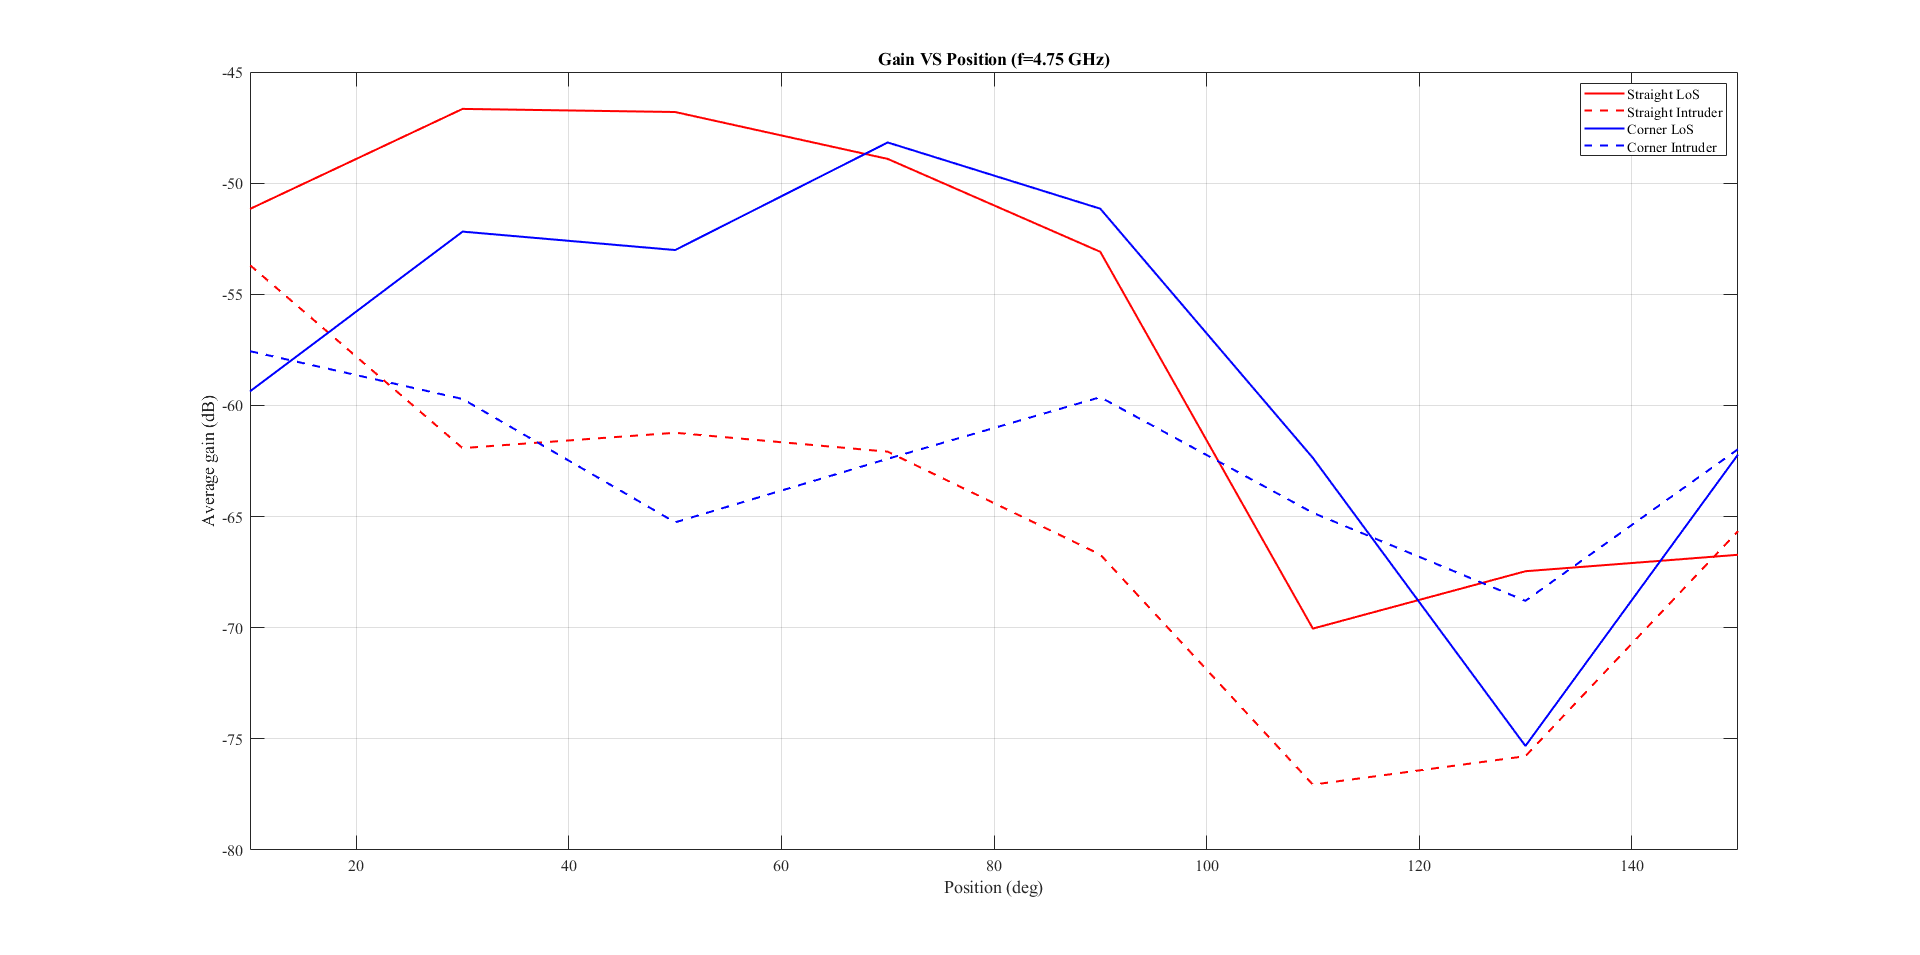
\includegraphics[width=1\textwidth]{figures/gain_vs_pos_475.png}
    \caption{Measured gain at $f=\SI{4.75}{\giga\hertz}$ each position for the four scenarios straight or corner-to-corner and with or without intruder.} 
    \label{fig:gain_vs_pos_475}
\end{figure}

The tests performed at $f=\SI{5.65}{\giga\hertz}$ show a more clear trend when comparing each test scenario. The intruder clearly dampens the input throughout the entire position spectrum until the final position \SI{150}{\degree}, indicating that this position is in a direction too far away from the transmitter to be influenced by the transmitted signal. The measured gain in all four test scenarios is close at this position. The difference between the measurement with and without intruder is largest for the straight setup. The intruder was in the straight scenario a person, whereas in the corner-to-corner scenario the intruder was a table. This indicates that the size of the intruder affects the ratio of measured gains. Finally, the difference in the placement of the transmitter antenna can be most clearly seen without intruder, where the maximum gain is at \SI{50}{\degree} in the straight test scenario and at \SI{70}{\degree} in the corner-to-corner test. 

\begin{figure}[H]
    \centering
    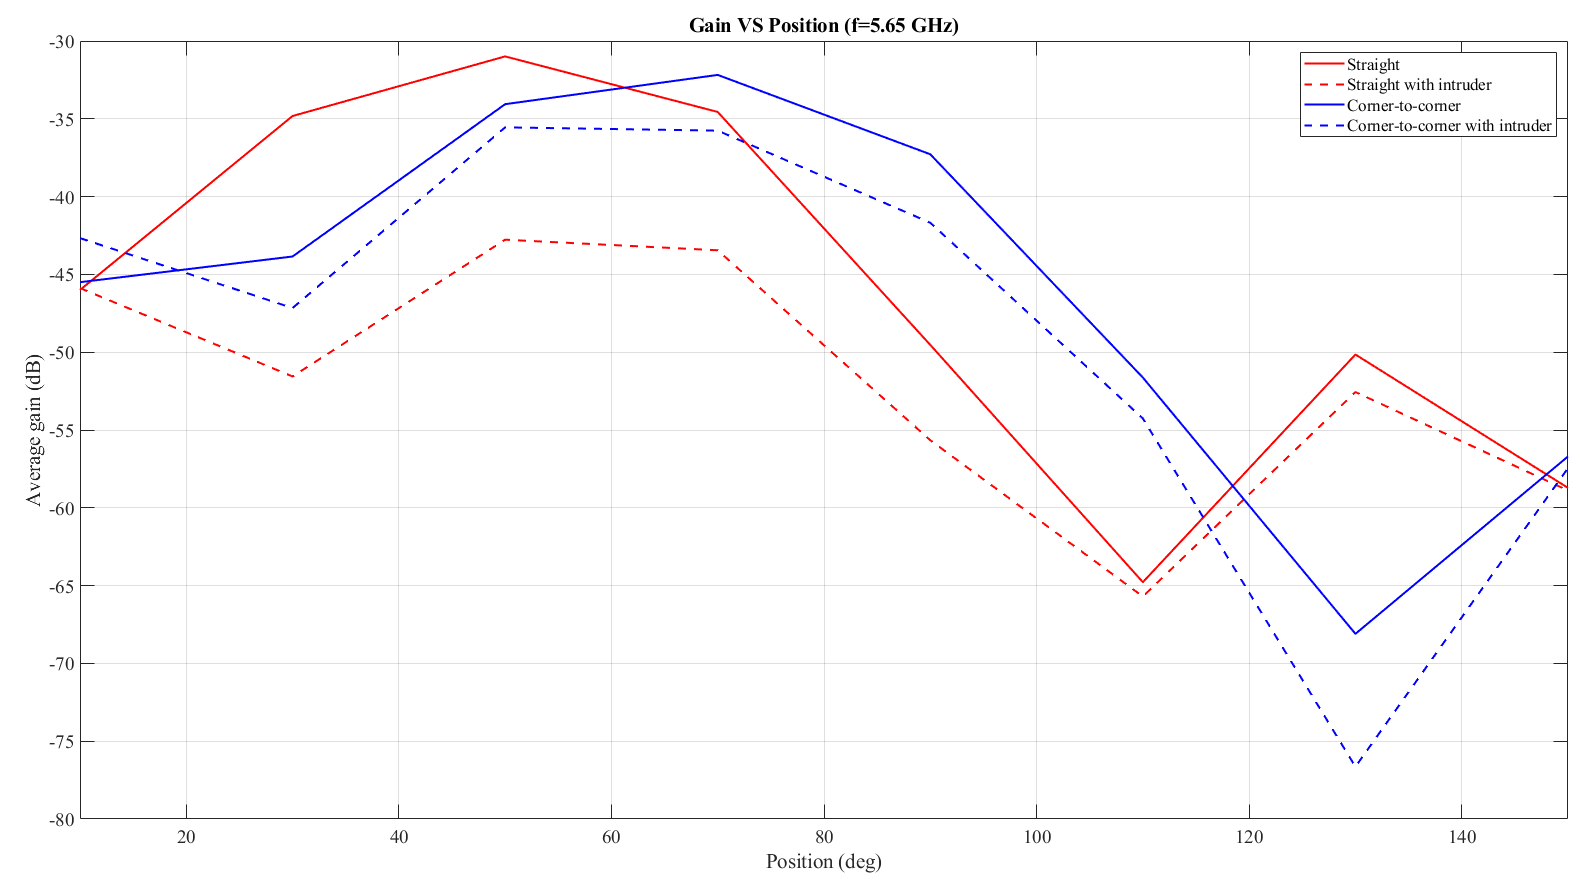
\includegraphics[width=1\textwidth]{figures/gain_vs_pos_565.png}
    \caption{Measured gain at $f=\SI{5.65}{\giga\hertz}$ each position for the four scenarios straight or corner-to-corner and with or without intruder.} 
    \label{fig:gain_vs_pos_565}
\end{figure}

The tests all show that at $f=\SI{5.65}{\giga\hertz}$ more power is received which is because, as shown in test of radiation pattern \ref{s:rad_test}, that the horn antenna has a higher gain at this frequency than at the lower frequency tested. 

While the turntable is turning the cable connected to the horn antenna will move with it. This will affect the phase of the signal. However, since the purpose of the test is to measure magnitude, this error is will not effect the test result. The test of the setup with a person as intruder is subject to measurement inaccuracies due to minimal movement.